\documentclass[10pt,a4paper,twoside]{article}
\usepackage[utf8]{inputenc}
\usepackage{hyperref}
\usepackage[a4paper,top=1cm,bottom=1.5cm,left=1cm,right=1cm]{geometry}
\usepackage{amsmath}
\usepackage{graphicx}

\author{Michele Veronesi}
\date{A.A. 2019/2020}
\title{Reti e Sicurezza}

\renewcommand*\contentsname{Indice}

\begin{document}
\pagenumbering{roman}
\maketitle
\tableofcontents
Gli argomenti segnati con * non sono stati trattati a lezione nel A.A. 2019/2020, vengono inseriti poiché presenti nelle domande di MEGA.
\newpage
Questo PDF è da usare in preparazione all'esame in quanto è un mix tra quanto detto da Marchiori (prevalentemente) e il libro (nei punti in cui la spiegazione del prof non era sufficiente). È improbabile che si riescano a capire gli argomenti da zero leggendo solo questo, è necessario aver seguito le lezioni e/o letto il libro.
\section*{Introduzione}
Le reti sono progettate inserendo vari livelli di astrazione. Esistono due modelli di riferimento: \textbf{ISO/OSI} e \textbf{TCP/IP}. Il secondo è quello su cui si basa internet.

\subsection*{ISO/OSI}
\begin{center}
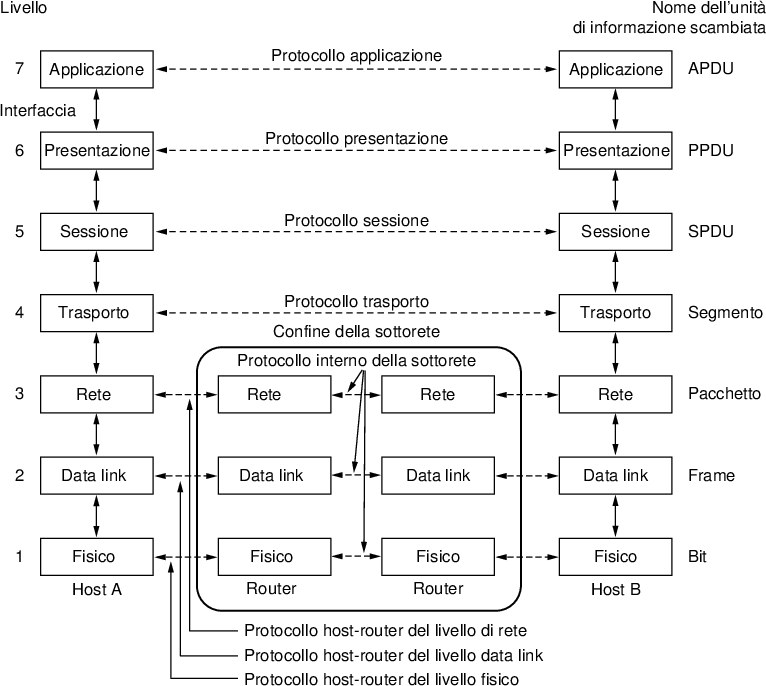
\includegraphics[width=0.7\textwidth]{images/iso_osi.png}
\end{center}
È lo standard di rete per eccellenza, tuttavia non è mai stato realizzato interamente nella pratica poiché ricerca ed investimento sono avvenute in tempi diversi. Il primo livello fisico si occupa di immettere i bit nel mezzo trasmissivo. Successivamente il livello data link si occupa di trasmettere i dati tra due host vicini nella topologia di rete, facendo eventualmente gestione degli errori. Salendo nell'astrazione troviamo il livello di rete, che si occupa di instradare i pacchetti in un percorso end-to-end tra due host della rete. Poi c'è il livello di trasporto, che ha il compito di consegnare il segmento al giusto processo in esecuzione nella macchina. Sessione e presentazione sono inutili, infine c'è il livello applicazione che interagisce con l'utente.

\subsection*{TCP/IP}
\begin{minipage}{0.4\textwidth}
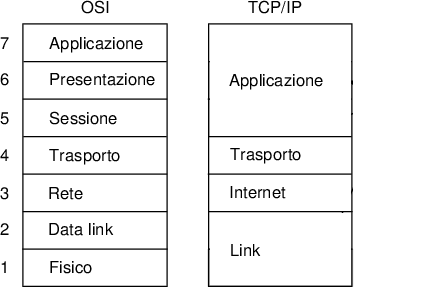
\includegraphics[width=\textwidth]{images/tcp_ip.png}
\end{minipage}
\begin{minipage}{0.6\textwidth}
Nella pratica si è deciso di unificare livello fisico e data link, rompendo la purezza dello standard. Inoltre il livello applicazione ha inglobato i due sottostanti, dunque le applicazioni gestiscono il mantenimento della sessione e la presentazione dei dati all'utente, scelta ragionevole.
\end{minipage}\\\\\\
Si analizzerà un modello ibrido, ovvero TCP/IP con livelli data link e fisico separati.

\newpage
\pagenumbering{arabic}

\section{Livello fisico}
Questo è il livello più basso. Definisce gli aspetti elettrici, di temporizzazione e le altre modalità con cui i bit, sotto forma di segnali elettromagnetici, vengono spediti sui canali di comunicazione.
\subsection{Serie di fourier}
Qualsiasi funzione periodica, sufficientemente regolare (ad esempio un segnale) f(t) può essere ottenuta sommando un numero (anche infinito) di funzioni seno e coseno. Questa somma è la serie di Fourier.\\
Più addendi (armoniche) si aggiungono in questa somma, migliore sarà la ricostruzione della funzione (segnale) originale. Già con 8 armoniche la ricostruzione del segnale è fedele all'originale. A frequenze più alte è possibile inviare più armoniche contemporaneamente, avendo quindi una ricostruzione del segnale più fedele.

\subsection{Attenuazione - Dispersione - Nyquist/Shannon}
Nessun mezzo di trasmissione è in grado di trasmettere segnali senza perdere parte dell'energia durante il processo. Se tutte le componenti di Fourier fossero attenuate uniformemente il segnale risulterebbe ridotto in ampiezza, facendo sorgere dunque il problema 
dell'\textit{attenuazione}.
Si misura in decibel ed è uguale a $10\cdot log_{10}(potenza\_trasmessa/potenza\_ricevuta)$\\
L'intervallo delle frequenze trasmesse senza una forte attenuazione è chiamato \textit{bandwidth} del canale, ed è una sua proprietà fisica.\\
Il \textit{teorema di Nyquist} afferma che il data-rate massimo è $2\cdot B\cdot log_2(L)$ dove B è la bandwidth del canale e L sono i livelli del segnale utilizzati per formare la funzione (nel caso del telegrafo L=2, 0 o 1). Tuttavia vale solo in condizioni ideali.\\
Nella realtà esiste il rumore. Il rapporto tra segnale (S) e rumore (N) si misura in decibel ed è\\$SNR=10\cdot log_{10}(\frac{S}{N})$ (Signal-Noise Ratio) e dipende dalla qualità del mezzo trasmissivo.\\
Il \textit{teorema di Shannon} tiene conto del rumore ed afferma che $max\_data\_rate=B\cdot log_2(1+\frac{S}{N})$\\\\
Nel caso in cui le componenti di Fourier non siano attenuate uniformemente si parla di \textit{dispersione}, un problema molto più grave che deteriora all'aumentare della frequenza e della distanza percorsa dal segnale. Qui c'è perdita d'informazione, dunque non è un problema risolvibile al livello fisico con un mezzo trasmissivo comune.\\
Una possibile soluzione è inserire ripetitori prima che il segnale si deteriori in maniera irreparabile.\\
Una soluzione migliore è l'uso dei solitoni, i quali funzionano come un elastico con un twist che si propaga su una corda, immuni alla dispersione. Se due solitoni si incontrano non succede nulla, ognuno continua per la sua strada, dunque sarebbero automaticamente risolti gran parte dei problemi delle reti che verranno analizzati in seguito.

\subsection{Basi della comunicazione}
La bandwidth (larghezza di banda) è misurata in data rate (misura del livello data link) ed è l'insieme di frequenze che trasmettiamo sul canale misurato in hertz Hz (misura del livello fisico).\\
Il data rate si può esprimere in
\begin{itemize}
\item \textit{bit rate}: quanti bit si trasmettono al secondo (bps)
\item \textit{baud rate}: si differenzia dal bitrate perché ad un simbolo (carattere o dato) possono corrispondere più bit nel caso in cui si utilizzino tecniche di modulazione del segnale non binarie, ad esempio modulazione di ampiezza, frequenza o fase. In questi casi la velocità bps può essere multipla di quella espressa in baud
\end{itemize}
La quantità d'informazione trasmessa dipende dal materiale del canale e dal segnale da trasmettere. Bisogna trovare il giusto equilibrio tra alte e basse frequenze, poiché se voglio mandare segnali a potenza doppia alla stessa distanza mi serve il quadrato della potenza.\\
$bit\_rate=(baud\_rate)\cdot (n\_bit\_in\_un\_simbolo)=(baud\_rate)\cdot log_2(L)$ dove $L$ è il numero di simboli dell'alfabeto utilizzato (telegrafo $L=2$).

\subsection{Vari tipi di cavo e confronto}
\begin{itemize}
\item \textit{twisted pair}: due cavi magnetici annodati tra loro per annullare il campo magnetico (crosstalk) coperti da una guaina protettiva. Più volte i cavi si incrociano e maggiore è l'annullamento del campo magnetico. La categoria del doppino indica la qualità del cavo, dunque maggiore è la categoria, migliore è l'annullamento del campo magnetico e quindi maggiore il numero di incroci dei cavi.
	\begin{itemize}
	\item UTP unshielded twisted pair - non schermato: cat. 3 doppino telefonico, cat. 5 usato in cavi ethernet.
	\item STP shielded twisted pair - schermato
	\end{itemize}
\item \textit{cavo coassiale}: composto da un nucleo conduttore coperto da un rivestimento isolante, a sua volta circondato da un conduttore cilindrico solitamente realizzato con una calza di conduttori sottili, che infine è avvolto da una guaina protettiva di plastica.\\
Schermatura migliore del doppino, dunque banda molto più larga, usato infatti per trasmissioni TV.
\item \textit{Fibra ottica}: capello di vetro con spessa protezione per evitare la rottura. Un solo cavo può contenere uno o più capelli di vetro.\\
Può essere di tipo multimodale se i fasci di luce rimbalzano, permettendo di multiplexare il canale semplicemente cambiando l'angolatura con cui si trasmette, oppure monomodale se i fasci di luce procedono in linea retta.\\
Vi sono diversi modi per connettere le fibre ottiche:
\begin{itemize}
	\item connettori: come nei cavi in rame, c'è una perdita del 10-20\%
	\item allineatori meccanici: si perde un 10\%
	\item fusione: metodo migliore e permanente, si perde circa l'1\%
\end{itemize}
Più costoso e delicato dei precedenti. Molto più sicuro poiché è difficile intromettersi nel canale (man in the middle a livello fisico praticamente impossibile). Inoltre offre molta più banda rispetto al cavo in rame.\\
La trasmissione non dipende solo dal micro tubo ma anche dal tipo di luce utilizzata: Laser o LED. Un laser permette di trasferire più dati per una distanza maggiore, mentre il LED è più economico e meno soggetto agli sbalzi di temperatura.
\end{itemize}

\subsection{Mezzi trasmissivi wireless}
In alternativa all'uso delle trasmissioni cablate si può usare lo spettro elettromagnetico per inviare segnali attraverso lo spazio (anche nel vuoto), dividendo segnali diversi in diverse zone dello spettro.\\
Le bande di frequenze sono propietarie (assegnate in base a un'asta o al beneficio che può trarne una tecnologia), Tranne per la banda ISM (Industrial Scientific Medical), cioè una banda libera e utilizzabile da chiunque ne necessiti. Questa è distribuita a pezzi per tutto lo spettro, così da coprire le necessità di uso si frequenze specifiche.\\
Il numero delle oscillazioni di un'onda è chiamato frequenza, e si misura in Hz (Hertz). La distanza tra due massimi o minimi consecutivi è la lunghezza d'onda e si indica con lambda ($\lambda$).\\
La maggior parte delle trasmissioni usa un'unica banda di frequenze ristretta per ottenere una migliore ricezione, ma in certi casi si usa la banda larga in tre modi:
\begin{enumerate}
\item spettro distribuito a frequenza variabile, in cui il trasmettitore passa da una frequenza all'altra centinaia di volte al secondo (comunicazioni militari);
\item spettro distribuito a sequenza diretta: fa uso di una codifica per dividere la banda, ad esempio il CDMA;
\item UWB (ultra wideband): trasmette i dati tramite segnali brevi in una banda estremamente ampia (usato nelle PAN - personal area network).
\end{enumerate}
I tipi di onde sono:
\begin{itemize}
\item \textbf{Onde radio:} sono omnidirezionali, quindi non necessitano di particolari allineamenti tra trasmettitore e ricevente. La radio AM è a basse frequenze: le onde di attraversano bene gli ostacoli ma si disperdono più facilmente. Le onde FM sono ad una frequenza maggiore di quelle AM, dunque hanno bisogno di antenne direzionali e sono più facili da bloccare; in compenso hanno una minore dispersione nello spazio.
\item \textbf{Microonde:} Frequenze maggiori di 100 Mhz. Perdono l'omnidirezionalità e viaggiano approssimativamente in linea retta; è dunque più semplice focalizzare il segnale su un unico ricevente e inviarlo per distanze maggiori. Di contro necessitano di ripetitori, a causa della curvatura terrestre, non attraversano bene gli edifici e gli ostacoli in generale, comprese condizioni meteorologiche sfavorevoli.
\item \textbf{Infrarosso:} Dette anche onde millimetriche, per via della lunghezza d'onda, vengono utilizzate in dispositivi quali i telecomandi per la TV. Sono ancora più direzionali delle microonde e bloccabili con maggiore facilità. Uno dei maggiori vantaggi di queste onde è che sono molto economiche da generare, e contemporaneamente anche un mezzo di trasmissione molto sicuro, essendo difficili da intercettare data la loro natura direzionale.
\item \textbf{Onde luminose:} L'utilizzo delle onde luminose come mezzo di comunicazione è stato usato molto frequente nel corso della storia. Al giorno d'oggi la frequenza della luce visibile è utilizzata per dispositivi quali i laser, che permettono di focalizzare il segnale su un unico ricevente anche molto distante, il grande problema di questa frequenza è che è facilmente bloccabile: basta una semplice foschia presente nell'atmosfera.
\end{itemize}

\subsection{Satelliti - caratteristiche e confronto}
I satelliti sono un mezzo di trasmissione broadcast per natura. Per evitare che tutti vedano la trasmissione viene adottata la crittografia.\\
La tipologia di un satellite si distingue in base alla sua posizione rispetto alle due fasce di Van Allen. Sotto la prima vi sono i LEO, tra la prima e la seconda i MEO, dopo la seconda i GEO.

\subsubsection{LEO - Low Earth Orbit}
Sono quelli meno costosi da mandare in orbita poiché non devono attraversare le fasce di Van Allen. Hanno una bassa latenza e ruotano attorno alla Terra molto velocemente.\\
Esempi di sistemi composti da satelliti LEO sono:
\begin{itemize}
	\item Iridium: 48 satelliti che coprono l'intera superficie terrestre usati per comunicazioni telefoniche. Caratterizzati da comunicazione intra-satellitare, dunque meno interferenze. Il segnale dal telefono satellitare va al satellite più vicino e viaggia nello spazio fino al satellite più vicino al ricevente.
	\item Global star: il segnale arriva al satellite più vicino che lo immette nella rete telefonica terrestre. Tramite questa arriva al satellite più vicino al destinatario. Meno costosa e composta da meno satelliti.
\end{itemize}

\subsubsection{MEO - Medium Earth Orbit}
Maggiore è l'altitudine di posizionamento minore sarà la velocità di rotazione, mentre cresceranno costi per lanciarli nello spazio e latenza.\\
Un esempio di sistema MEO è il GPS. Un suo miglioramento è A-GPS (Assisted GPS) che sfrutta la rete telefonica per ridurre il tempo di fix.

\subsubsection{GEO - Geostationary Earth Orbit}
L'unica orbita geostazionaria terrestre è sopra l'equatore. Visto che la distanza minima tra i satelliti è di 2 gradi ve ne sono al massimo 360/2=180.\\
Sono praticamente fermi, muovendosi ad una velocità minima. Vengono dunque usati fare foto satellitari, televisione via satellite e in generale tutti gli usi che richiedono questa caratteristica.

\subsection{Modulazione digitale}
Processo di conversione tra bit e segnali che li rappresentano.
Vi sono due tipologie:
\begin{itemize}
\item \textit{trasmissione in banda base (baseband transmission)}: i segnali occupano frequenze che vanno da 0 a un massimo che dipende dal tasso di trasmissione
\item \textit{trasmissione in banda passante (passband transmission)}: il segnale occupa una banda di frequenze attorno a quella del segnale portante. Usato nel wireless e nella fibra ottica.
\end{itemize}

\subsubsection{Trasmissione in banda base}
La tecnica più naturale per effettuare questa tecnica si chiama \textit{NRZ} (non ritorno a zero) consiste nell'assegnare una tensione positiva per l'1, una negativa per lo 0 (nella fibra presenza/assenza di luce).\\
In questo modo il segnale potrebbe oscillare tra i livelli positivi e negativi ogni 2 bit (in caso di alternanza 0/1). Avremo bisogno perciò di una banda di almeno B/2 Hz, dove B è il bit rate (Nyquist - limite fisico insuperabile).\\
Una possibile strategia è di usare più di 2 livelli per il segnale in modo da avere un baud rate più alto del bit rate.\\
Un altro problema di NRZ è che in caso di attenuazione o distorsione è difficile distinguere una sequenza di simboli uguali vicini. Una soluzione è usare il \textit{clock recovery}, ovvero miscelare il segnale di clock con quello originale tramite XOR. Il clock effettua una transizione ad ogni bit, in questo modo procede al doppio del bit rate. Una tecnica clock recovery è la \textit{codifica di Manchester}, ed è molto costosa in termini di overhead (richiede il doppio della banda rispetto a NRZ).\\
Per fare un passo indietro e trovare un compromesso si può usare \textit{NRZI} (NRZ invertito), ovvero produrre un cambio di fase ogni volta che cambia il bit da trasmettere.\\
Tuttavia lunghe sequenze di 0 sono ancora un problema. Un codice ben conosciuto che lo risolve si chiama \textit{4B/5B}, che tramite una tabella nota sostituisce sequenze di 4 bit con sequenze di 5 bit, che causa un overhead del 25\%.\\
Un'altra tecnica è lo \textit{scrambling}, il quale fa una XOR tra una sequenza pseudocasuale (segnale bianco, che tende ad avere la sua energia ben distribuita) ed il segnale da trasmettere. Non c'è overhead.

\subsubsection{Trasmissione in banda passante}
Collocare un segnale in una certa banda di frequenza è utile per permettere a diversi tipi di segnali di coesistere sullo stesso canale.\\
Il valore assoluto della frequenza non influenza la capacità di trasferimento dati. Possiamo quindi prendere un segnale in banda base e traslarlo in una banda passante senza perdita di informazioni.\\
Questo processo è ottenuto modulando un segnale portante che risiede in banda passante; ci sono 3 tecniche:
\begin{itemize}
\item \textit{ASK (amplitude shift keying - AM)}: due diverse ampiezze sono usate per rappresentare 0 e 1. Generalizzando si possono associare N ampiezze ad N simboli. Molto semplice da mettere in pratica ma molto sensibile ai disturbi.
\item \textit{FSK (frequency shift keying - FM)}: si possono usare due o più frequenze da a associare a due o più simboli. Meno sensibile ai disturbi (migliore qualità), richiede meno energia per effettuare la trasmissione, è complesso da mettere in pratica e occupa più banda.
\item \textit{PSK (phase shift keying)}: l'onda portante è sistematicamente traslata di 0 o 180 gradi all'inizio della trasmissione di ogni simbolo. Ha delle varianti:
	\begin{itemize}
	\item \textit{BPSK (binary PSK)}: quando vi sono 2 simboli nell'alfabeto utilizzato (esempio 0 e 1).
	\item \textit{QPSK (quadrature PSK)}: fa uso di 4 traslazioni per trasmettere 2 bit di informazioni per simbolo.
	\end{itemize}
\end{itemize}
Per trasmettere più bit per simbolo si possono combinare più tipi di modulazione tenendo la frequenza costante (semplificando la generazione del segnale e la sincronizzazione) e mescolando ampiezza e fase (two gusti is meglio che one). In questo modo, dalle 4 variazioni di fase del QPSK, aggiungendo la modulazione in ampiezza, otteniamo \textit{QAM-16 e QAM-64 (quadrature amplitude modulation)}. Si possono usare QAM di ordine superiore, tuttavia la probabilità di errore aumenta notevolmente poiché i simboli nel constellation diagram sono molto più vicini.\\
Per associare sequenze di bit ai simboli dei vari QAM o QPSK di usa il \textit{Gray code}, che li associa in modo tale che simboli adiacenti differiscano di un solo bit (in modo da favorire la correzione ai livelli superiori).

\subsubsection{Modulazione delta}
Usato in D-AMPS (2G). Invece che rappresentare tutti i dati si rappresenta solo la differenza di ampiezza nel tempo. Utile nel telefono poiché la frequenza vocale non varia di molto.
Se il segnale sale si inserisce un 1, se scende 0. In questo modo c'è perdita d'informazione, poiché la variazione memorizzata non è precisa.

\subsection{Multiplexing}
I canali trasmissivi vengono normalmente condivisi da più segnali. Si effettua perciò il \textit{multiplexing} del canale, che può essere fatto a divisione di tempo, frequenza o codice.

\subsubsection{FDM - Multiplexing a divisione di frequenza}
Ad ogni utente vengono assegnate frequenze diverse. Il segnale generato viene traslato nelle frequenze assegnate (FSK). Viene usato nelle trasmissioni radio AM, dove si varia l'ampiezza (ASK) ma la frequenza resta costante.
Viene inoltre usato nelle ADSL.\\
FDM viene di fatto utilizzato in tutte le parti di internet e veniva usato anche nel telefono: la struttura gerarchica della prima rete telefonica lo usava per gestire più telefonate.\\
Quando vengono inviati solo dati digitali è possibile dividere lo spettro in maniera più efficiente senza usare le bande di guardia. \textit{OFDM (orthogonal FDM)} divide la banda del canale in molte sottoportanti che inviano dati in maniera indipendente. Viene usata in 802.11, TV via cavo e linee elettriche.\\
Nella fibra ottica prende il nome di WDM (wavelength division multiplexing), poiché non si basa su frequenze ma su lunghezza d'onda della luce, ma la logica resta uguale.

\subsubsection{TDM - Multiplexing a divisione di tempo}
Gli utenti fanno a turno secondo una politica di scheduling round-robin. Il tempo è diviso in slot. Si può usare con FDM poiché usa pochi simboli.\\
È più semplice da realizzare, tuttavia richiede sincronia e quindi necessita di tempi di guardia. Ha la possibilità di dividere il canale in infinite parti, tuttavia aumenta l'overhead e diminuisce la velocità all'aumentare della divisione.

\subsubsection{CDM - Multiplexing a divisione di codice}
Introdotto nel terzo standard del 2G (\textit{CDMA - Code Division Multiple Access}), trascende dal concetto di divisione in base alla frequenza e al tempo: tutti spediscono sulla frequenza che vogliono quando vogliono. Si distinguono i mittenti con la teoria dei codici. I codici sono assi che formano uno spazio multidimensionale (tante dimensioni quanti mittenti). Ogni parola sta nell'asse corrispondente. Per distinguere 1 e 0 nei diversi codici, dividiamo l'asse in parte positiva e negativa. Per rendere il sistema efficiente usiamo solamente due simboli: 1 per la parte positiva, -1 per quella negativa (rappresenta lo 0).\\
Al momento della trasmissione viene fatta la somma tra tutti i simboli. Per estrarre il messaggio desiderato, il ricevente esegue il prodotto scalare con le matrici di Hadamard proiettando il segnale sull'asse d'interesse.\\
La peculiarità di queste matrici è che sono composte da 1 e -1. Le righe sono mutuamente ortogonali.\\
Si formano in questo modo (costruzione di Sylvester) dove k è il numero di righe che avrà la matrice (dunque il numero di mittenti che devono condividere il canale:
\begin{equation}
H_{2^k}=
\begin{bmatrix}
H_{2^{k-1}} & H_{2^{k-1}}\\
H_{2^{k-1}} & -H_{2^{k-1}}
\end{bmatrix}
=H_2 \otimes H_{2^{k-1}}
\end{equation}
dove $\otimes$ indica il prodotto di Kronecker tra matrici.\\
Le righe della matrice sono mutuamente ortogonali (prendendo due righe qualunque sono ortogonali), ogni riga rappresenta la \textbf{chip sequence} associata ad un mittente. Quest'ultimo per inviare un 1 invia la sua sequenza, per un -1 la sua negazione.\\
Le righe iniziali sono 1 1, 1 -1.\\\\
\textbf{Esempio (k=1):}
\begin{equation}
H_2=
\begin{bmatrix}
1 & 1 \\
1 & -1
\end{bmatrix}
\end{equation}
In questo caso i due assi sono 1,1 e 1,-1, dunque vi sono due mittenti. Alla ricezione del segnale si esegue il prodotto scalare con un asse e in base al risultato si ricava l'informazione. Se il segnale ricevuto è 2, 0, facendo il prodotto scalare con il primo asse si avrà $1\cdot 2+1\cdot 0=2>0$, dunque il primo mittente ha inviato un 1, visto che il risultato è positivo. Se fosse stato 0 non avrebbe trasmetto nulla, se fosse stato negativo avrebbe trasmesso un -1 (ovvero 0).\\
Volendo verificare cos'ha trasmesso il secondo mittente facciamo $2\cdot 1 + 0\cdot (-1)>0$, dunque anche lui ha mandato un 1.\\
Infatti entrambi hanno inviato il loro chip, i quali si sono sommati automaticamente.\\

\subsection{Linee xDSL}
ADSL sta per \textit{Asymmetric Digital Subsriber Line}. Questo nome deriva dal fatto che queste linee vengono usate per collegare gli utenti al sistema pubblico telefonico previa stipulazione di un contratto a pagamento. Trasmettono completamente in digitale. Il problema principale è che la qualità del segnale decade esponenzialmente all'aumentare della lunghezza dell'ultimo miglio, se quest'ultimo è composto da cavo UTP. Per questo motivo si sta provvedendo a sostituire i cablaggi in rame con più efficiente fibra ottica.\\
Inizialmente il sistema era progettato per portare segnale telefonico, dunque frequenze entro i 4000 Hz. Per permettere il passaggio di segnali QAM digitali si è rimosso il filtro all'ingresso dell'abitazione, e aggiunto uno splitter in corrispondenza dell'apparecchio telefonico per dividere le frequenze. Il canale è quindi multiplexato con FDM nel modo riportato in figura.
\begin{center}
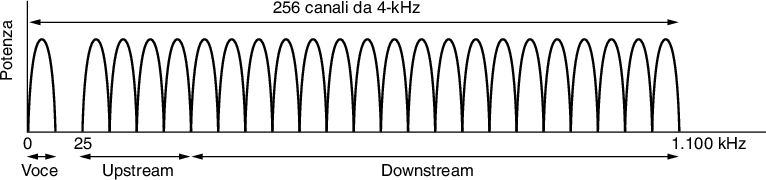
\includegraphics[width=0.7\textwidth]{images/multiplexing_adsl.png}
\end{center}
Viene diviso in 256 parti ognuna da 4000 Hz, 1 per la voce, 5 vuoti, 32 upstream e il resto downstream.\\
Usando tutti i canali larghi uguali è possibile usare la stessa tecnologia trasmissiva usata nel canale telefonico moltiplicata per 256 canali.\\
Viene usato OFDM, visto che i dati sono completamente digitali.\\
La conversione da analogico a digitale e viceversa viene effettuata dal \textit{modem - modulator demodulator}, che si colloca tra il computer (digitale) e il sistema telefonico (analogico).

\subsection{Switching - commutazione}
La rete telefonica pubblica ha una struttura gerarchica. Ogni telefono è connesso tramite il local loop alla centrale locale dell'operatore telefonico. Questa a sua volta è connessa alla centralina urbana, che di fatto è connessa con le altre tramite centraline interurbane. Quando un utente richiede la connessione con un altro, di fatto viene creato un canale tra i due. Una volta questo lavoro veniva fatto manualmente dalle centraliniste, ora vi sono 3 tecniche automatizzate.
\begin{itemize}
\item \textbf{Commutazione di circuito:} usata agli albori, è l'automatizzazione del lavoro delle centraliniste, viene di fatto creato un canale fisico. Vi è un ritardo iniziale per questo processo, tuttavia la connessione sarà molto stabile.
\item \textbf{Commutazione di messaggio:} Quando un messaggio arriva ad uno switch si crea il passaggio. Il cammino si crea al passare del messaggio iniziale.
\item \textbf{Commutazione di pacchetto:} come la precedente, solamente che il messaggio viene spezzato in pacchetti se è troppo grande per la memoria degli switch. Riduce il problema dei colli di bottiglia.
\end{itemize}

\subsection{Sistema telefonico mobile}
\subsubsection{0G - IMTS}
Derivato diretto del PTT (push-to-talk), canale half-duplex (trasmissione e ricezione non possibili contemporaneamente).\\
Successivamente nasce \textit{IMTS}, che ha un canale full-duplex, implementa protocolli per la privacy, in modo da non sentire comunicazioni altrui, utilizza trasmettitori ad altissima potenza che coprono un raggio di 100 km con 23 canali (troppo limitativo). Usato ancora in luoghi sperduti.

\subsubsection{1G - AMPS e TACS}
Usa celle che coprono un raggio di 10-20 km, dunque aumenta la capacità di utenti e diminuisce la potenza necessaria per trasmettere alla cella, ottenendo quindi telefoni cellulari di dimensioni ridotte.\\
Per evitare l'interferenza tra celle adiacenti, si usa FDM, usando da 3 a 7 frequenze diverse.\\
La cella ha al centro la stazione base (switching center) connessa al sistema telefonico pubblico.\\
Ogni cellulare ha un numero seriale di 32 bits più 10 numeri per il numero telefonico (34 bits). Ogni 15 minuti circa manda in broadcast i suoi 32+34 bits per registrarsi alla cella più vicina.\\
Quando si effettua una chiamata si invia una richiesta tramite l'apposito canale condiviso. In ricezione c'è il \textit{canale di paging} (condiviso) che i cellulari ascoltano costantemente per sapere se ci sono chiamate in arrivo per loro.\\
La gestione del passaggio di cella (\textit{handoff}) viene fatta interamente dalle stazioni base: quando il segnale è troppo debole il provider chiede alle celle vicine quanta potenza ricevono da quel cellulare, che viene assegnato a quella con la potenza più alta.\\
Questa tecnica prende il nome di \textit{hard handoff} poiché avviene un troncamento (seppur breve) della connessione.\\
Per rimediare a questo problema si può attuare un \textit{soft handoff}, in cui il cellulare si sgancia dalla vecchia cella dopo essersi agganciato a quella nuova. Per realizzarlo è necessario che il cellulare abbia la capacità di connettersi a due celle contemporaneamente. Questa tecnica viene introdotta solamente nel 3G.

\subsubsection{2G - D-AMPS e GSM}
La vera differenza dalle precedenti generazioni è il passaggio al digitale. D-AMPS (USA) è retrocompatibile con AMPS. Tuttavia le onde del 2G sono a frequenze più alte, dunque le onde sono più corte. La densità delle celle nel territorio aumenta e ai cellulari bastano antenne più piccole per ricevere il segnale.\\
Trasmettendo in digitale è possibile comprimere i dati, ad esempio usando la \textit{modulazione delta} (descritta sopra).
Le comunicazioni compresse vengono gestite con TDM. La qualità del suono è peggiorata, tuttavia non è rilevante in una comunicazione telefonica.\\\\
GSM (Europa) differisce di poco da D-AMPS. I suoi canali sono più larghi ma ce ne sono meno. Si è preferita la qualità rispetto alla quantità.\\
Un'altra differenza sta nella gestione dell'handoff: il controllo della qualità del segnale è decentralizzato ai cellulari. Sarà compito di questi ultimi inviare una richiesta di handoff quando si accorgono di essere troppo distanti. Questa tecnica prende il nome di \textit{MAHO (Mobile Assisted HandOff)}. Per misurare la potenza del segnale si sfruttano i "tempi morti" del TDM, ovvero quando non è il nostro turno di trasmettere.\\
Vi sono 4 tipi di celle:
\begin{itemize}
\item Macro: molto grandi, sopraelevate con 35 km di raggio.
\item Micro: più piccole, posizionate sul tetto degli edifici.
\item Pico: molto piccole, usate per aree con molte persone, anche indoor.
\item Umbrella: piccola estensione dell'apparato usata per "tappare buchi" tra le celle principali.
\end{itemize}
Con il 2G viene inoltre introdotta la \textit{SIM (Subscriber Identity Module)} che contiene IMSI (ID univoco della SIM) e KI (chiave di autenticazione che ne impedisce la duplicazione).\\
\begin{itemize}
\item Il cellulare invia IMSI in chiaro
\item L'operatore risponde con una sequenza casuale
\item Il cellulare firma la sequenza con la KI e la rimanda alla cella
\item L'operatore verifica la firma
\end{itemize}

\subsubsection{2.5G - GPRS ed EDGE}
GPRS è un overlay del 2G che permette di trasmettere anche dati internet. Il problema è che il 2G è pensato per le trasmissioni voce e dunque la connessione dati web tende ad occupare un intero canale voce anche quando il traffico dati è ridotto.\\
È il primo standard ad introdurre il passaggio da message switching a packet switching, dunque le tariffe vengono calcolate in base al numero di pacchetti inviati per la prima volta.\\
In GPRS i canali internet e voce vengono allocati dinamicamente in base alla richiesta (dando priorità alla voce).\\
Vi sono differenti tipi di classi di GPRS:
\begin{itemize}
\item Classe C: richiede un settaggio manuale del canale da utilizzare (GSM o GPRS)
\item Classe B: la scelta del canale è automatica
\item Classe pseudo A: le due tipologie di connessioni sono aperte contemporaneamente ma in un singolo canale
\item Classe A: le due connessioni sono aperte contemporaneamente su due canali diversi
\end{itemize}
EDGE è un'evoluzione del GPRS che migliora la trasmissione dei dati.

\subsubsection{3G - CDMA}
Offre un data rate maggiore e supporta più utenti contemporaneamente grazie all'utilizzo di bande di frequenza più larghe. Ci sono 2 standard principali:
\begin{itemize}
\item W-CDMA (Wideband CDMA): utilizzato in Europa e Giappone, conosciuto anche come UMTS
\item CDMA-2000: utilizzato negli USA, usa bande più strette e ha più canali rispetto al precedente, avendo quindi una minore velocità di trasmissione.
\end{itemize}
L'utilizzo di CDMA per multiplexare il canale richiede che la cella riceva segnali non attenuati, dunque se un cellulare è più distante dalla cella dovrà aumentare la potenza di trasmissione, impattando sulla durata della batteria.

\subsubsection{3.5G - HSPA+}
\begin{itemize}
\item HSDPA (High Speed Download Packet Access) (H) è un'evoluzione dell'UMTS retrocompatibile, migliora la velocità in download.
\item HSUPA (Hig Speed Upload Packet Access) migliora la velocità in upload (non ha mai visto la luce perché sorpassato da H+).
\item HSPA+ (High Speed Packet Access+) (H+) migliora la velocità sia in upload che in download.
\end{itemize}

\subsubsection{4G - HSOPA}
HSOPA (High Speed OFDM Packet Access), detto anche LTE. Ha bande variabili, usa sempre più banda e tecniche aggiuntive di FDM e TDM. Utilizzando più banda si è sconfinato nelle frequenze del digitale terrestre; ciò richiede agli utenti di quest'ultimo di installare un filtro sull'antenna per bloccare le interferenze.

\subsection{Nuove trasmissioni radio}
Con l'arrivo delle radio stereo si è posto il problema della retrocompatibilità con quelle mono. Le trasmissioni vengono effettuate su un canale pilota in cui si avvisa una radio stereo della presenza dei nuovi canali stereo. I due segnali sinistro (S) e destro (D), vengono ricreati attraverso un nuovo canale M=(S+D)/2. In aggiunta viene creato un nuovo canale E=(S-D)/2 che indica la differenza. In questo modo le radio stereo ricostruiscono S e D a partire da M ed E. Tuttavia porta ad un deterioramento della qualità peggiorando il rapporto segnale/rumore. Dunque la qualità sonora risulterà migliore nel segnale mono.\\
Negli ultimi anni è stata anche introdotta la DAB (Digital Audio Broadcasting), grazie alla quale è possibile trasmettere più stazioni e con maggiore precisione (meno interferenza). Presenta tuttavia problemi di interferenza con apparecchi domestici e perdita d'informazione dovuta alla compressione audio.

\section{Livello data link}
Il livello data link si occupa di gestire il flusso di dati tra due host vicini nella rete. Inoltre effettua controllo e a volte correzione dell'errore.
\subsection{Framing}
 Per farlo, considera gruppi di bit come frame. Per effettuare questa suddivisione vi sono 4 modi: conteggio dei byte, byte stuffing, bit stuffing e violazione della codifica del livello fisico (non trattato).
\begin{itemize}
\item  \textbf{Character count:} Si utilizza un header per specificare il numero di caratteri che costituisce il payload. Tuttavia basta un singolo errore al livello fisico o la perdita di sincronia per sfasciare tutta la sequenza di header.
\item \textbf{Byte stuffing:} Si utilizza un \textit{flag byte} all'inizio e alla fine di ogni frame per identificarne i limiti. Per evitare che questa sequenza compaia all'interno del payload causando danni si usa un metodo di escaping, ovvero si interrompe il realizzarsi della sequenza inserendone un'altra. Il ricevente, che conosce la sequenza di limitazione del frame, sa che se sta per realizzarsi subito dopo c'è un carattere di escape, che andrà a rimuovere poiché non significativo.
\item \textbf{Bit stuffing:} Esattamente come il byte stuffing solamente fatto a livello di bit.
\end{itemize}

\subsection{Error detection}
Per effettuare questa operazione è necessario introdurre il concetto di \textit{distanza di hamming}: due messaggi (di lunghezza uguale) sono distanti n se differiscono di n bit. Esistono diverse tecniche: bit di parità, checksum e CRC.

\subsubsection{Parity bit}
Ogni $m$ bit inseriamo uno 0 se i bit a 1 sono pari, 1 altrimenti. In questo modo i bit a 1 sono sempre pari.\\
Con questa tecnica possiamo avere un bit flippato ogni $m$ bit. Qualunque sia $m$, presi due messaggi diversi, la loro codifica sarà distante almeno 2.\\
Possiamo quindi avere un errore ogni $m+1$ bits, ovvero possiamo identificare un error rate di $\frac{1}{m+1}$.\\
Il data rate si riduce invece a $\frac{m}{m+1}$ (per trasmettere $m$ bit ne servono $m+1$).\\
Il codice più forte si ha con $m=1$, tuttavia il data rate è dimezzato (pessima cosa).\\
Per difendersi dagli \textit{errori burst}, che flippano molti bit vicini, il parity bit cosi com'è non è sufficiente. Si adotta quindi la tecnica dell'\textit{interleaving}, ovvero si calcola il parity bit delle colonne invece che delle righe. Se i bit di parità delle righe della matrice qui sotto sono (0 1 1) quelli delle colonne sono (0 0 0). In questo modo, anche se un'intera riga venisse distrutta, è possibile accorgersene con un parity bit 3. L'alternativa è cambiare la sequenza trasmissiva da righe a colonne (inversione della matrice). Se prima la sequenza da trasmettere era 110 001 111 diventa 101 101 011.
\begin{equation}
\begin{matrix}
1 & 1 & 0\\
0 & 0 & 1\\
1 & 1 & 1
\end{matrix}
\end{equation}

\subsubsection{Checksum}
Con checksum si intende un gruppo di bit di controllo associati al messaggio. Parity bit aggiunge un checksum di 1 bit. Metodi più potenti prevedono l'uso di somme progressive dei bit di dati del messaggio in complemento a uno. Gli errori possono essere rilevati sommando l'intera parola contenete sia i bit di dati che il checksum: se il risultato è 0 allora non è stato rilevato alcun errore.

\subsubsection{CRC - Cyclic Redundancy Check}
Questo metodo si basa sull'aritmetica polinomiale in base due, $GF[2]$.
Ogni sequenza di bit è vista come un polinomio, ad esempio 1011 diventa $x^3+x+1$, 110010 diventa $x^5+x^4+x$. Operazioni che prima venivano fatte su bit ora vengono effettuate su polinomi. In particolare, in $GF[2]$, la somma è uguale alla sottrazione, ovvero equivalgono a fare l'operazione logica XOR bit a bit. Ad esempio $1011\pm 0101=1110$.
\paragraph{Procedimento} Si sceglie un polinomio generatore $G(x)$ che sarà il divisore della divisione.\\
Abbiamo un messaggio $M(x)$, che sarà il dividendo. Calcoliamo quindi il resto $R(x)$ svolgendo la divisione tra polinomi. Infine si fa una XOR tra $M(x)$ e $R(x)$, si trasmette quindi il risultato.\\
Tuttavia l'entità del resto potrebbe essere più grande del messaggio effettivo, più cresce il grado di $G(x)$ più messaggi non sono divisibili. La soluzione è moltiplicare $M(x)$ per $x^{deg(G(x))}$.\\
Diciamo $r=deg(G(x))$ e $G(x)=x^r+x^{r-1}+...+x^0$, quindi $P(x)=M(x)\cdot x^r$. In questo modo si ottiene sempre un resto più piccolo del messaggio originale.\\
Dal punto di vista dei bit, moltiplicare un polinomio per $x^r$ equivale a fare lo shift a sinistra di $r$ posizioni.\\
Dunque nella pratica la divisione è fatta tra $M(x)\cdot x^{deg(G(x))}$ e $G(x)$. Seguono poi le operazioni prima descritte.\\
Per il \textit{decoding} basta rimuovere il resto con una XOR e fare di nuovo lo shift a destra di $r$ posizioni per rimuovere il fattore $x^r$ aggiunto al messaggio originale.\\
Per accorgersi dell'errore (se avvenuto) si fa in questo modo:\\
abbiamo ricevuto $x^r\cdot M(x)+R(x)$ che equivale a $x^r\cdot M(x)-R(x)$. Abbiamo dunque un polinomio divisibile per G(x) poiché è stato tolto il resto. Basterà effettuare quindi la divisione tra i bit ricevuti e lo stesso polinomio generatore, se il resto è 0 non c'è stato errore.\\
La potenza di questo metodo dipende dal polinomio generatore scelto e dal tipo di errore.
\begin{itemize}
\item Per rilevare \textit{errori singoli}, se il polinomio di errore è $E(x)=x^i$ basterà che G(x) abbia 2 o più termini.
\item Per rilevare \textit{errori doppi}, con $E(x)=x^i+x^j$, basta che $G(x)$ non sia divisibile per questi due fattori.
\item Per rilevare \textit{errori in numero dispari}, ovvero $E(x)$ ha un numero dispari di monomi, basta che $x+1$ sia fattore di $G(x)$. Dimostrazione:\\
$G(x)=(x+1)\cdot P1(x)$ quindi $G(1)=0\cdot P1(1)=0$ perché $x+1=1+1=0$\\
$E(x)\% G(x)=0 \iff G(x)\cdot P2(x)=E(x)$ | ovvero $E(x)$ è divisibile per $G(x)$\\
$\iff (x+1)\cdot P1(x)\cdot P2(x)=E(x)$\\
$E(1)=0\cdot P1(1) \cdot P2(1)=0$\\
$E(x)=x^i+x^j+...+x^0$ con numero dispari di componenti\\
$E(1)=1$ ASSURDO! ($1 \neq 0$)
\item Per rilevare \textit{errori burst} di lunghezza $j+1$ basta che $deg(G(x))>j$
\end{itemize}
Riassumendo, scegliere il polinomio generatore con +1 alla fine, meglio se irriducibile (senza divisori).\\
All'aumentare del grado di $G(x)$ irriducibile la potenza aumenta in modo esponenziale. La probabilità di fallimento è $(\frac{1}{2})^{deg(G(x))}$, ovvero decresce esponenzialmente all'aumentare del grado.
\paragraph{Esempio} Si calcoli il CRC di 10011101 usando $G(x)=x^4+x+1$\\
\begin{minipage}{0.5\textwidth}
- $M(x)=x^7+x^4+x^3+x^2+1$\\
- $P(x)=M(x)\cdot x^{deg(G(x))}=x^{11}+x^8+x^7+x^6+x^4$\\
- Divido $P(x)$ per $G(x)$ e calcolo il resto $R(x)$\\
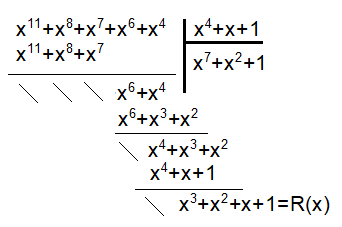
\includegraphics[width=0.6\textwidth]{images/divisione.png}
\end{minipage}
\begin{minipage}{0.5\textwidth}
- Eseguo la XOR tra $P(x)$ e $R(x)$\\\\
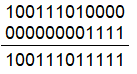
\includegraphics[width=0.3\textwidth]{images/xor.png}\\
Il risultato è il dato da trasmettere.
\end{minipage}
\\\\
Per effettuare il decoding basterà rimuovere il resto, riottenendo dunque $P(x)$, 100111010000, ed eseguire lo shift a destra di $deg(G(x))$, 10011101.\\
Per verificare la presenza di errori si effettua la divisione tra i bit ricevuti visti come polinomio e $G(x)$, verificando il resto. Infatti $(x^{11}+x^8+x^7+x^6+x^4+x^3+x^2+x+1)/(x^4+x+1)$ ha resto 0, dunque non c'è stato errore.

\subsubsection{Built-in Error Detection}
In molti casi l'informazione extra per effettuare error detection fa parte dei dati stessi, in questo modo viene fatta indipendentemente dal metodo di trasmissione.
\paragraph{Codice di Luhn} Viene applicato alle carte di credito, analogo al parity bit code ma in base 10. L'ultimo numero delle carte di credito dipende dai precedenti 15 ed è calcolato tramite questo algoritmo:
\begin{itemize}
\item Si raddoppiano le cifre in posizione dispari (contando da destra a sinistra)
\item Si sommano le singole cifre (attenzione, non i numeri)
\item La cifra di Luhn è quanto manca per raggiungere il successivo multiplo di 10 a partire dalla somma ottenuta.
\end{itemize}
Viene usato anche nell'IMEI del telefono.\\
In generale tutti i codici a barre e qr-code hanno un sistema di controllo built-in (diverso da Luhn).

\subsection{Error correction}
In questi codici si riporta il messaggio sbagliato al più vicino corretto con distanza di Hamming minore.
\subsubsection{Repetition code}
Nel repetition code $R_n$ ogni bit si ripete $n$ volte (es. $R_3$: 010 $\rightarrow$ 000 111 000).\\
Per due diversi messaggi, le loro rispettive codifiche in $R_n$ sono distanti almeno $n$, quindi con $R_n$ possiamo trovare fino a $n-1$ errori. Il data rate con questa tecnica diminuisce drasticamente a $\frac{1}{n}$ (per trasmettere un bit ne trasmetto $n$).\\
Se abbiamo un codice i cui messaggi corretti sono distanti almeno $n$ e intervengono $k$ errori, riusciamo a tornare al messaggio originale solo se $k<\frac{n}{2}$.

\subsubsection{Codici di Hamming}
Un codice di Hamming($x,y$) significa che codifica $y$ bits usandone $x$ in totale.
\paragraph{Hamming(7,4)} In questo caso ci sono 3 bit di protezione ogni 4 bit di dati.\\
Da $2^7=128$ combinazioni possibili ho solamente $2^4=16$ messaggi corretti, le altre servono per error correction e detection. I bit extra si dividono equamente la parità dei bit di dati.\\
\begin{minipage}{0.25\textwidth}
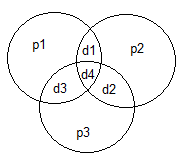
\includegraphics[]{images/hamming.png}
\end{minipage}
\begin{minipage}{0.75\textwidth}
$p_n$ sono i bit di protezione, $d_n$ i bit dati.\\
$p_1$ protegge $d_1, d_3, d_4$;\\$p_2$ protegge $d_1, d_2, d_4$\\$p_3$ protegge $d_2, d_3, d_4$
\end{minipage}\\\\
La matrice $G$ di protezione è
\begin{equation}
G=
\begin{bmatrix}
1 & 0 & 0 & 0 &|& 1 & 1 & 0\\
0 & 1 & 0 & 0 &|& 0 & 1 & 1\\
0 & 0 & 1 & 0 &|& 1 & 0 & 1\\
0 & 0 & 0 & 1 &|& 1 & 1 & 1
\end{bmatrix}
\end{equation}
composta da la matrice identica $I_y$ e la matrice dei bit di parità. Quest'ultima è cosi composta: la prima colonna rappresenta $p_1$, a seguire $p_2$ e $p_3$; le righe rappresentano i bit di dati, la prima $d_1$, a seguire gli altri fino a $d_4$. Se c'è un 1 in posizione ($i,j$) significa che il bit $d_i$ è protetto dal bit $p_j$.\\
Il codice di Hamming è un codice lineare, questi ultimi hanno delle particolari proprietà.

\paragraph{Proprietà codici lineari (teorema del peso minimo)} Ogni messaggio ha un \textit{peso}, ovvero quanti bit a 1 contiene.\\
Se il peso minimo dei vettori riga della matrice generatore $G$ in un codice ($x,y$) è $z$\\
Allora ogni coppia di messaggi legali ha distanza minima $z$ e il codice si indica con ($x,y,z$). In particolare $z=x-y$.\\
In questi codici si potrà fare error detection fino a $z-1$ errori, error correction fino a $\frac{z-1}{2}$ errori.\\
Il data rate di Hamming(7,4,3) è $\frac{4}{7}\simeq 0,57=57\%$. Confrontato ad un $R_3$, che ha lo stesso livello di protezione e un data rate $\frac{1}{3}\simeq 0,33=33\%$, riusciamo a vedere i benefici di questi codici.\\\\
Per l'error detection si fa moltiplicazione con la matrice di parità $G$. Se il risultato è diverso da 0 c'è errore.\\
Per l'error recovery basta portarsi al messaggio corretto più vicino.\\\\
Per gestire gli \textit{errori burst} è necessario applicare il metodo della matrice invertita spiegato nel parity bit. Il prezzo da pagare è quello di avere un buffer che tenga i dati ricevuti per poi riordinarli al termine della trasmissione.

\subsubsection{Codici di Reed-Solomon}
Questi codici sono basati sull'aritmetica polinomiale come CRC.\\
Vengono usati per correggere segnali della sonda spaziale Voyager, che trasmette con una potenza bassissima ad una distanza lunghissima.\\
Godono delle stesse proprietà dei codici lineari, ovvero un RS($x,y$) corregge fino a $\frac{x-y-1}{2}$.\\
La vera differenza sta che usano i bytes come unità di misura, non i bits.\\
Inoltre riescono a fronteggiare le \textit{erasures}, un problema molto più grave del normale bit flippato, che consiste nella scomparsa di dati. Un RS($x,y$) corregge fino a $x-y$ erasures.\\
Errori ed erasures possono essere corretti contemporaneamente, ma gli errori contano il doppio delle erasures. In particolare $2\cdot errori+erasures<x-y$, questo perché per erasures non serve fare detection.

\subsubsection{Limite di shannon}
\begin{center}
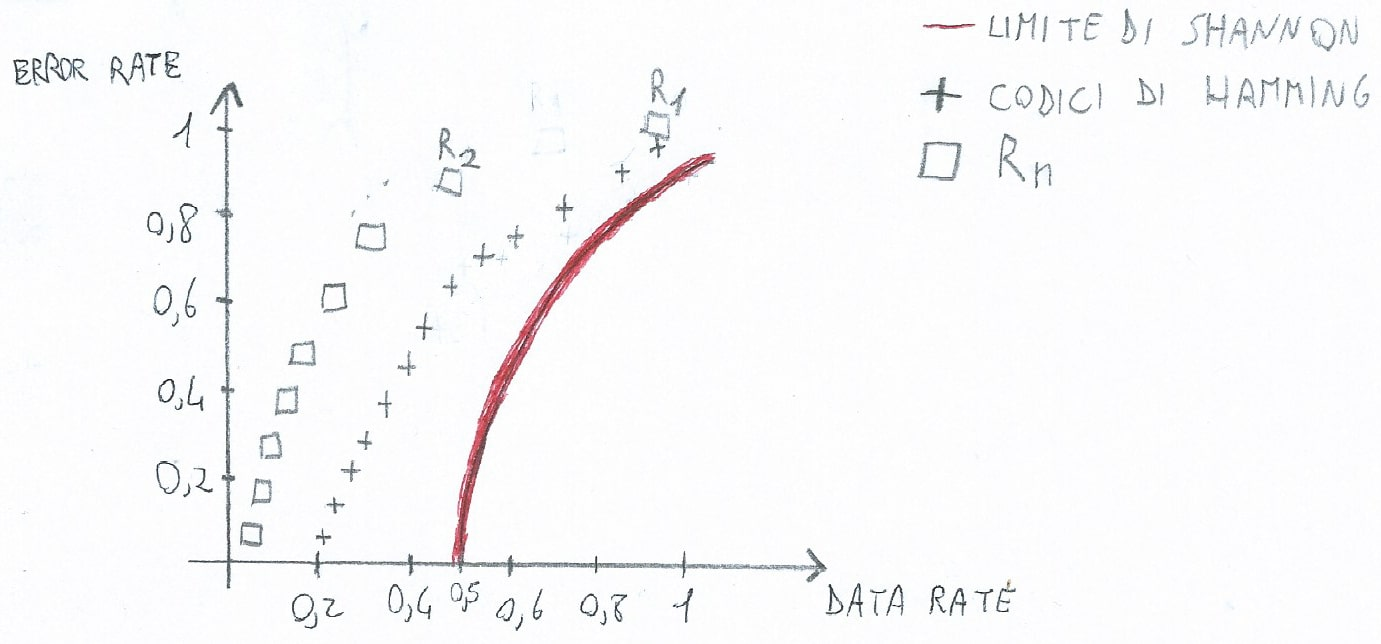
\includegraphics[width=0.6\textwidth]{images/shannon.jpg}
\end{center}
Dal grafico (tralasciando i dettagli) notiamo che c'è una discesa logaritmica aumentando la potenza di $R_n$, dunque non si ottiene una notevole riduzione di error rate al calare del data rate. Notiamo anche che i codici di Hamming seguono la stessa curvatura leggermente spostata verso destra, ovvero abbattono l'error rate ma perdono comunque troppo data rate.\\
Shannon ha dimostrato che la curva dei codici riesce ancora ad avere un data rate positivo (50\%) anche se si fa tendere l'error rate a 0. Tuttavia non esiste un codice che raggiunga tale limite.

\subsubsection{Codice a controllo di parità a bassa densità}
\textit{LDPC - Low Density Parity Check} è un codice in cui i bit di protezione creano un grafo in cui si scambiano informazioni. Il grafo comprende sia bit di controllo che bit di dati. Si dice "a bassa densità" poiché questo grafo ha poche connessioni.\\
La potenza di questo codice si avvicina al limite di Shannon, il problema del decoding dei dati è però NP-completo, ovvero molto lento.

\subsection{Gestione dei flussi}
In un canale semplice, se inviamo troppi dati rischiamo di generare un collo di bottiglia e conseguente perdita dei dati. È necessario definire protocolli che stabiliscano le regole di comunicazione tra due hosts in modo da arginare il problema.

\subsubsection{Protocolli stop-and-wait}
Con questa tecnica viene inviato un blocco di dati e si aspetta un messaggio di conferma (\textit{acknowledgment -ACK}), il quale segnala che la trasmissione è andata a buon fine e si è in attesa del prossimo frame.\\
Il vantaggio principale di questo protocollo è che basta un canale half-duplex, visto che non c'è mai comunicazione contemporanea.\\Tuttavia c'è il grande svantaggio dell'attesa (wait), che porta ad un enorme spreco di tempo, e quindi di banda.\\
Un piccolo miglioramento potrebbe essere quello di spedire l'ACK di ritorno solo se il frame passa l'error control e inserire un timeout nel mittente, allo scadere del quale si considera fallita la trasmissione.\\
Sarà necessario inoltre aggiungere informazioni per il controllo del flusso, ovvero numerare i frame per evitare i duplicati. Visto che la trasmissione è seriale e non parallela, basterà un bit per il numero di frame in modo da distinguere l'alternanza.\\
Un esempio di protocolli stop-and-wait sono \textit{PAR e ARQ}, applicati in canali full-duplex duplicando il protocollo ad ogni lato della linea. Tuttavia portano ad un overhead pazzesco, solamente per inviare gli ACK la banda dimezza.

\subsubsection{Piggyback}
Il canale di trasmissione la maggior parte delle volte è full-duplex, dunque mentre riceviamo possiamo attaccare in piggyback (letteralmente cavallina) l'ACK al prossimo frame che dobbiamo inviare. In questo modo c'è una minimizzazione dell'overhead. È necessario però stare attenti a non far scattare il timer del mittente: se non abbiamo nessun frame da inviare entro questo lasso di tempo, bisogna inviare un frame apposito per l'ACK. Per questo motivo abbiamo una notevole diminuzione di overhead solo se la comunicazione è equilibrata, altrimenti la situazione peggiora.\\\\
Il canale però è ancora sottoutilizzato in termini di tempo. Abbiamo un round trip delay (RTD), ovvero il tempo che trascorre dalla trasmissione del frame all'arrivo del suo ACK, troppo alto. Aumentare la banda non risolverebbe il problema, infatti l'utilizzo della linea in caso di protocolli con ACK è $\frac{S}{S+C\cdot R}$, dove $S$ è la lunghezza dei frame in bits, C la larghezza di banda in bit/s, R è l'RTD. Se $S<C\cdot R$ abbiamo un'efficienza $<50\%$.\\
La soluzione a questo problema è parallelizzare la trasmissione.

\subsubsection{Sliding windows}
Questa tecnica sfrutta l'idea del parallelismo sopra introdotta. Invece che attendere un ACK per ogni frame, ne attendiamo uno per ogni $n$ frame, dove $n$ è una potenza del 2 per motivi implementativi. L'idea è appunto quella di una \textit{finestra scorrevole}: tanto più è aperta tanti più pacchetti inviamo senza bisogno di conferma.\\
L'apertura massima della finestra coincide con $n$, tuttavia se superiamo l'apertura di $\frac{n}{2}$ sorgono problemi di perdita di sincronia per sovrapposizione di stati tra cicli diversi della finestra del ricevente, che potrebbe considerare una ritrasmissione come un nuovo frame.\\
Sia mittente che destinatario hanno una finestra. All'inizio quella del mittente è completamente chiusa, poiché non ha ancora inviato nulla, quella del destinatario è aperta al massimo (misura definita dal protocollo implementato). Il mittente invia frame finché la sua finestra non raggiunge l'apertura massima. Nel frattempo il destinatario riceve questi frame ed invia i rispettivi ACK, in piggyback o meno. Ogni volta che invia un ACK chiude di uno scatto la finestra e apre lo scatto successivo per ricordarsi che quel frame lo ha ricevuto e ne sta aspettando un altro. Il mittente, al ricevimento dell'ACK, fa la stessa cosa: chiude la fetta di finestra relativa al frame confermato e ne apre un'altra, inviando un nuovo frame.

\subsubsection{Protocolli go-back-n}
La taglia della sliding window di chi riceve è 1, dunque riceve serialmente. Il trasmittente ha una sliding windows di taglia maggiore di 1, diciamo $n$, dunque lo fa parallelamente.\\
Questa tecnica porta a vantaggi quando non ci sono molti errori ma il prodotto $bandwidth \cdot RTD$ è alto.\\
È necessario che il mittente tenga una copia degli $n$ frame di cui la relativa finestra è aperta (quelli inviati ma di cui non è stato ricevuto l'ACK), servirà dunque un buffer di taglia $n$ frames, insieme ad altri $n$ timer per l'eventuale ritrasmissione in assenza di ACK. Il nome dei protocolli deriva dal fatto che se in una sequenza di $n$ frame ne viene perso anche solo 1 è necessario ritrasmetterli tutti, infatti in caso di errore si attende non viene ritornato l'ACK relativo al frame perso, dunque dopo lo scattare del timeout il mittente ricomincierà a trasmettere dall'ultimo frame confermato.
\begin{center}
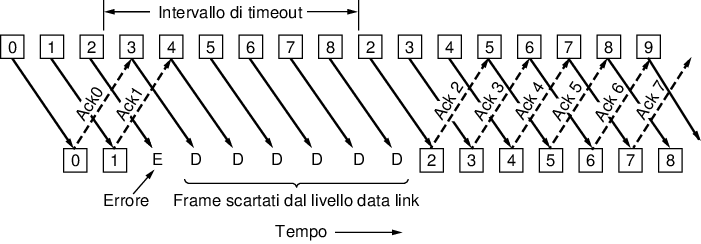
\includegraphics[width=0.7\textwidth]{images/go_back_n.png}
\end{center}

\subsubsection{Selective repeat}
In questo caso anche il ricevente applica il parallelismo, dunque anch'esso deve avere un buffer per contenere gli $n$ frame della sequenza.\\
Una miglioria al protocollo è l'introduzione di una risposta \textit{NAK} (ACK negativo) inviata in caso di frame corrotto non correggibile. Il mittente che riceve NAK effettua la ritrasmissione anche se non è scaduto il timer a partire dal numero del frame indicato.
Un'altra possibile ottimizzazione è quella di inviare un ACK ogni $tot$ frame ricevuti contenente il numero dell'ultimo frame arrivato. Tutti i frame con numero $<=$ a quello contenuto nell'ACK saranno considerati ricevuti.
\begin{center}
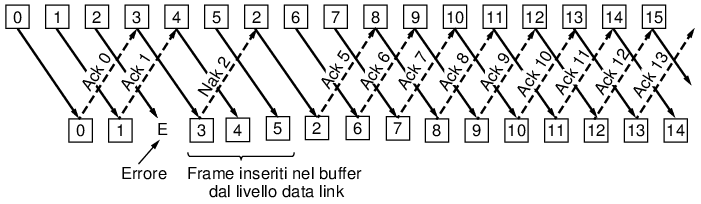
\includegraphics[width=0.7\textwidth]{images/selective_repeat.png}
\end{center}

\subsection{Esempi di protocolli reali}

\subsubsection{HDLC - High level Data Link Control}
Protocollo ancora in uso in alcuni modem, fax e bancomat; sviluppato da IBM. I frame sono delimitati da bit stuffing.\\
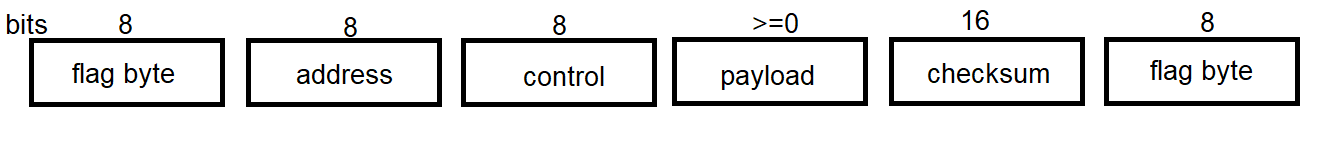
\includegraphics[width=\textwidth]{images/hdlc.png}\\
Checksum: calcolato con CRC-16\\
Address: componente di indirizzamento, usato se ci sono terminali multipli dentro la stessa rete (cluster). Nelle grandi reti va fatto a livello superiore.\\
Utilizza sliding window con 3 bit ($2^3=8$ spicchi, parallelismo massimo 4).\\
Esistono 3 tipi di frame: information, supervisory e unnumbered. Variano per il campo control.
\paragraph{Frame information} Il campo control è composto da:\\
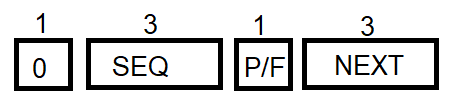
\includegraphics[width=0.4\textwidth]{images/hdlc_information.png}\\
Il primo bit a 0 identifica un frame di tipo information.\\
SEQ: indica il numero all'interno della sliding window.\\
P/F: gestisce inizio e fine trasmissione.\\
NEXT: è l'ACK in piggyback.

\paragraph{Frame supervisory} Si occupa della supervisione del flusso di dati\\
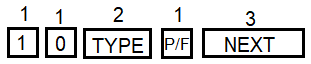
\includegraphics[width=0.4\textwidth]{images/hdlc_supervisory.png}\\
I primi due bit, rispettivamente a 1 e 0, indicano questo tipo di frame.\\
Type 0: ACK - receive ready\\
Type 1: Reject (NAK generalizzato), ritrasmetti tutto ciò che era nella sliding window\\
NEXT: Indica il primo frame da rimandare in caso di reject\\
Type 2: Receive not ready (segnala congestione), la trasmissione è bloccata fino all'arrivo di un ACK (type 0)\\
Type 3: Selective reject (classico NAK), richiede la ritrasmissione di un singolo frame indicato in NEXT.\\
Non esiste parallelismo.

\paragraph{Frame unnumbered} Usati per gestire la connessione\\
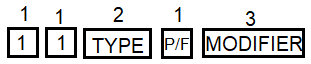
\includegraphics[width=0.4\textwidth]{images/hdlc_unnumbered.png}\\
I primi due bit a 1 identificano il frame unnumbered.\\
I campi type e P/F mantengono lo stesso significato, MODIFIER assume uno dei seguenti valori:\\
DISC: disconnect, segnala che la macchina sta uscendo dalla rete\\
SNRM: segnala che la macchina è appena entrata e richiede un canale asimmetrico, dove il nuovo entrato è meno importante, terminali stupidi (es. bancomat)\\
SABM: crea invece una connessione bilanciata asincrona, chi entra ha gli stessi diritti degli altri\\
FRMR: frame reject, è arrivato un frame non identificabile\\
UA: unnambered ACK, dedicato a questo tipo di frame\\
Non esiste parallelismo.

\subsubsection{PPP - Point-to-Point Protocol}
Protocollo usato nella rete internet.\\
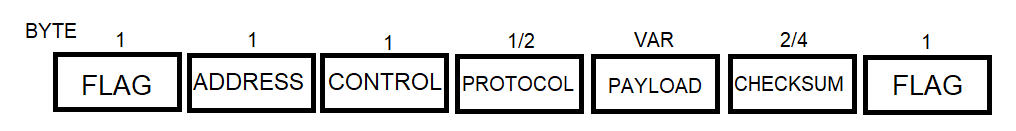
\includegraphics[width=\textwidth]{images/ppp.png}\\
Utilizza il byte stuffing (meno efficiente)\\
ADDRESS: non utilizzato, valore fisso a 11111111 (lasciato per retro compatibilità con HDLC)\\
CONTROL: controllo di flusso, non utilizzato, valore fisso a 00000011, non usa quindi numbering (sliding windows) e ACK\\
PROTOCOL: specifica il protocollo implementato, infatti PPP è un \textit{meta-protocollo}, ovvero il significato del payload dipende da questo campo.\\
CHECKSUM: utilizza CRC, dunque non fa error correction che viene lasciata ai livelli superiori.\\\\
PPP implementa due tipi di protocolli:
\begin{itemize}
\item \textit{LCP}: livello data link di negoziazione
\item \textit{NCP}: livello di rete
\end{itemize}
È inoltre utilizzato nelle ADSL. Qui è necessario stabilire la taglia massima del payload, ovvero l'\textit{MTU (Maximum Trasmission Unit)}.\\
Se questo parametro è troppo grande si avranno frame più grandi e quindi meno overhead, tuttavia c'è più probabilità che il frame venga corrotto se il canale non è abbastanza affidabile.\\
Al contrario, se è troppo piccolo, aumenta l'overhead e lo spreco di banda, necessario però se il canale è poco affidabile.\\\\
Esistono due varianti di PPP:
\begin{itemize}
\item PPPoE (over Ethernet)
\item PPPoA (over ATM)
\end{itemize}
Incapsulano frame PPP per essere inviati su Ethernet o ATM.\\
\textbf{ATM (Asynchronous Transfer Mode):} usa TDM, è analogo a HDLC, gestisce il controllo di flusso, la sliding window ha 4 bit (16 spicchi) ed è orientato alla connessione.

\section{Sottolivello MAC}
In qualsiasi rete broadcast il problema chiave è la scelta dell'entità che dovrà acquisire il diritto di utilizzo del canale in caso di competizione. Di questo se ne occupa \textit{MAC - Medium Access Control}, situato nell'astrazione tra livello fisico e data link.\\
Una possibilità per affrontare il problema è suddividere il canale staticamente per il numero di utenti. Tuttavia non è una soluzione accettabile, poiché il numero di utenti su Internet è altamente variabile. Inoltre ci sarebbe un enorme spreco di banda quando un utente non ha bisogno di trasmettere.\\
È necessario quindi allocare il canale dinamicamente secondo queste assunzioni:
\begin{itemize}
\item \textit{Traffico indipendente}: ci sono $N$ stazioni indipendenti che generano frame da trasmettere.
\item \textit{Canale singolo}: c'è solamente un canale per le $N$ stazioni.
\item \textit{Collisioni osservabili}: tutte le stazioni hanno la possibilità di accorgersi di una collisione tra frame.
\item \textit{Tempo continuo o diviso in intervalli}: si può supporre tempo lineare o suddiviso in \textit{slot}.
\item \textit{Rilevamento di portante}: le stazioni possono o meno rilevare se il canale è occupato prima di trasmettere.
\end{itemize}

\subsection{Protocolli ad accesso multiplo senza rilevamento della portante}
\subsubsection{ALOHA puro}
L'idea di base è quella di consentire agli utenti di trasmettere ogni volta che hanno da inviare dati, senza controllare se il canale è libero e senza controllare se avvengono collisioni. Se non si riceve l'ACK, si rimane in attesa per un intervallo di tempo casuale prima di ripetere la trasmissione.\\
La capacità di trasporto dei sistemi ALOHA è massima quando la dimensione dei frame è fissa.\\
La probabilità che $k$ frames siano generati durante un certo intervallo di tempo, se la comunicazione è bilanciata, è di tipo poissoniano, cioè se la media delle trasmissioni nell'unità di tempo è $G$, allora la probabilità che ci siano $k$ trasmissioni è data dalla \textit{distribuzione di Poisson}.\\
\begin{equation}
Pr[k]=(G^k\cdot e^{-G})/k!
\end{equation}

Affinché un frame non collida non devono essere generati altri frame nel suo tempo di trasmissione $G$ ne in uno slot precedente lungo $G$, poiché la coda del frame precedentemente spedito colliderebbe con la testa di quello in trasmissione. Definiamo $G$ come \textit{frame time} (tempo di trasmissione di un frame).\\
La probabilità di generare 1 frame ($k=1$) in due frame time ($2G$) è
\begin{equation}
S=(2G\cdot e^{-2G})/2!=G\cdot e^{-2G}
\end{equation}
Prendendo $G$ come variabile andiamo a trovare la derivata e il massimo della funzione.\\
$y=x\cdot e^{-2x}$\\
$y'=e^{-2x}+x\cdot e^{-2x}\cdot (-2)=e^{-2x}\cdot (1-2x)$\\
$e^{-2x}\cdot (1-2x)=0 \iff x=\frac{1}{2}$\\
In particolare $G=\frac{1}{2}=0.5$ è un massimo assoluto (non riporto lo studio del segno, fatelo voi sfaticati), quindi la capacità di trasporto massima si ha con questo valore, dunque si usa $S=\frac{1}{2e}=0.184\simeq 18\%$ del data rate.

\subsubsection{ALOHA slotted}
Un miglioramento dell'ALOHA puro è \textit{ALOHA slotted}, che introduce il concetto di suddivisione del tempo in intervalli discreti chiamati \textit{slot}, corrispondenti ad un frame time (tempo di trasmissione di un frame).\\
In questo modo quando un host vuole trasmettere deve attendere l'inizio del prossimo frame time, non interrompendo la trasmissione già in corso nello slot corrente.\\
Ora il periodo vulnerabile è dimezzato ed è $S=G\cdot e^{-G}$.\\
Sempre derivando la funzione e trovando il massimo, otteniamo $G=1$ come valore ottimale, quindi $S=\frac{1}{e}\simeq 36\%$ del data rate utilizzato, il doppio rispetto ad ALOHA puro.

\subsection{Protocolli ad accesso multiplo con rilevamento della portante}
Con ALOHA slotted si crea sincronia, poiché se durante uno slot più host diventano pronti alla trasmissione tutti quanti tenteranno di trasmettere all'inizio del successivo. Per migliorare le prestazioni è necessario desincronizzare gli host prima che la collisione avvenga.\\
Innanzitutto è utile che un host pronto alla trasmissione controlli se il canale è libero prima di cominciare. Tuttavia questo non è sufficiente, poiché due o più macchine potrebbero rilevare il canale libero e trasmettere comunque contemporaneamente.\\
Si introducono quindi il concetto di persistenza e i protocolli \textit{CSMA}.

\subsubsection{CSMA persistente e non persistente}
Il protocollo \textit{CSMA p-persistente} (Carrier Sense Multiple Access), dopo aver controllato se il canale è libero, trasmette con probabilità $p$. Dunque non trasmette con probabilità $1-p$. Se invece trova il canale occupato attende che sia libero e trasmette o meno con la stessa probabilità.
\begin{center}
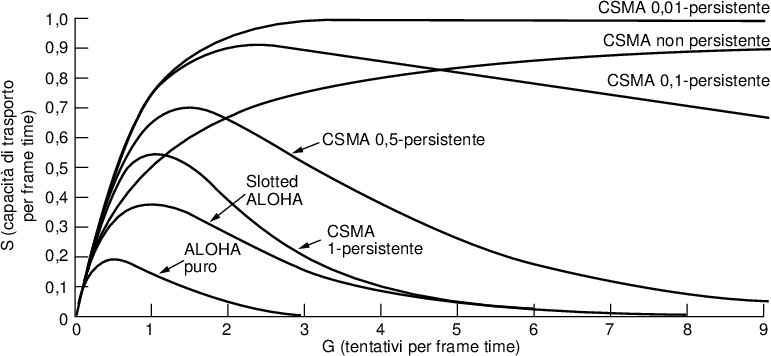
\includegraphics[width=0.6\textwidth]{images/csma.png}
\end{center}
Le prestazioni migliori le abbiamo con un bassissimo livello di persistenza, ovvero quando un host trasmette con probabilità all'1\% se trova il canale libero: CSMA 0.01-persistente riesce a raggiungere il 100\% di banda utilizzata nel suo massimo.\\
Tuttavia, sia ALOHA che CSMA p-persistente hanno una curva di decrescita costante una volta raggiunto il massimo della funzione.\\\\
CSMA non persistente, al contrario di tutti i protocolli visti fin'ora, in caso di canale occupato attende un tempo casuale e ricontrolla, invece che trasmettere con una certa probabilità. La sua peculiarità è quella di essere in costante crescita all'aumentare di $G$, dunque più utenti ci sono e meglio funziona. La banda utilizzata tende al 100\% ma non ci arriva mai, tuttavia è un compromesso accettabile per non avere una curva di decrescita all'aumentare degli utenti.\\\\
NB: È da notare che in tutte le formule e protocolli visti fin'ora non compare il numero degli utenti. Difatti quando si dice che un certo protocollo di accesso offre X\% banda del canale, si intende che ogni utente ha $\frac{X}{N}$ banda se nel sistema ci sono $N$ utenti.

\subsubsection{CSMA/CD - con rilevamento delle collisioni}
Questo protocollo è un'ottimizzazione dei CSMA visti precedentemente. Prende il nome di \textit{CSMA/CD (CSMA with Collision Detection)} poiché durante la trasmissione ascolta se avvengono collisioni verificando se varia l'onda in uscita rispetto a quella che dovrebbe essere. Nel caso in cui se ne accorga termina subito la trasmissione e attua le tecniche viste prima per assicurarsi il canale.\\
Per evitare di sprecare frame con dati significativi, prima di iniziare la trasmissione vengono lanciati "frame sonda" piccoli. La prima stazione che riesce a trasmettere uno di questi frame si assicura l'uso esclusivo del canale ed inizia a trasmettere frame con payload valido.
\begin{center}
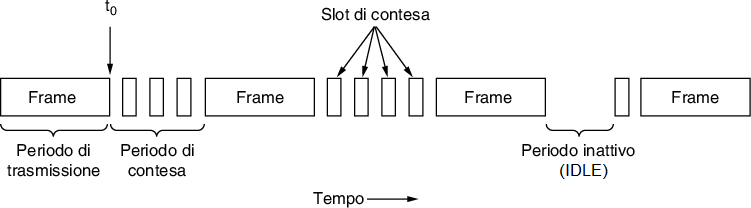
\includegraphics[width=0.7\textwidth]{images/csmacd.png}
\end{center}

\subsection{Protocolli senza collisione - CSMA/CA}
Le collisioni influenzano negativamente le prestazioni del sistema, soprattutto quando il prodotto $bandwidth\cdot RTD$ è alto.\\
Rendono il tempo di trasmissione variabile, cosa pessima nei sistemi real-time.\\
Da queste esigenze nasce quindi \textit{CSMA/CA (CSMA with Collision Avoidance)}.
In tutti i seguenti protocolli si suppone di avere esattamente $N$ utenti.

\subsubsection{Protocollo a mappa di bit}
In questo protocollo nel periodo di contesa non avvengono collisioni. Questo periodo viene diviso in $N$ parti, una per utente. Ogni utente invierà un bit a 1 nel suo slot assegnato se necessita di trasmettere qualcosa. Infine si assegna il canale in ordine in base agli utenti che hanno inviato un 1.
\begin{center}
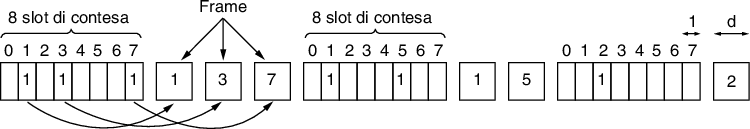
\includegraphics[width=0.6\textwidth]{images/mappabit.png}
\end{center}
Con questo metodo la durata del periodo di contesa dipenderà quindi dal numero di utenti. Sarà pertanto più efficiente a pieno carico, ovvero quando tutti gli utenti vogliono trasmettere: infatti con tanti utenti il contention period diventa lungo anche se uno solo vuole parlare.\\
In particolare, l'efficienza a pieno carico se la taglia del frame è $d$ bits è $\frac{d}{d+1}$.\\\\
La soluzione migliore è quella ibrida che unisce il meglio di CSMA/CD, che funziona bene con pochi host, e CSMA/CA che va meglio con molti utenti, nascono perciò i protocolli a contesa limitata.

\subsubsection{Protocollo token passing}
Un altro modo per assegnare turni di trasmissione è usando un \textit{token}, ovvero un breve messaggio che conferisce al ricevente l'accesso esclusivo al canale. Ogni stazione effettua la trasmissione e passa il gettone. È utile nelle reti ad anello.

\subsubsection{Protocollo binary countdown}
Una miglioria della mappa di bit è questo protocollo. Una stazione intenzionata a trasmettere comunica in broadcast il proprio indirizzo partendo dal bit più significativo (supponendo indirizzi di lunghezza uguale). Il vincitore è chi ha l'indirizzo più alto. Qui l'efficienza del canale è $d/(d+log_2N)$ dove $N$ è il numero di utenti. Se il formato del frame viene scelto con cura in modo che l'indirizzo del mittente costituisca il primo campo del frame l'efficienza raggiunge il 100\%.

\subsubsection{Prestazioni protocolli simmetrici}
Prima di introdurre i protocolli \textit{asimmetrici} (in cui le stazioni non sono tutte uguali) è necessario analizzare le prestazioni di quelli \textit{simmetrici} (ALOHA, CSMA, etc...). Il vero problema di questi ultimi è la competizione, infatti quando ci sono poche stazioni c'è alta probabilità di successo, all'aumentare di questi la banda si stabilizza ad una certa percentuale (ad esempio 36\% in ALOHA slotted - vedi grafico).
\begin{center}
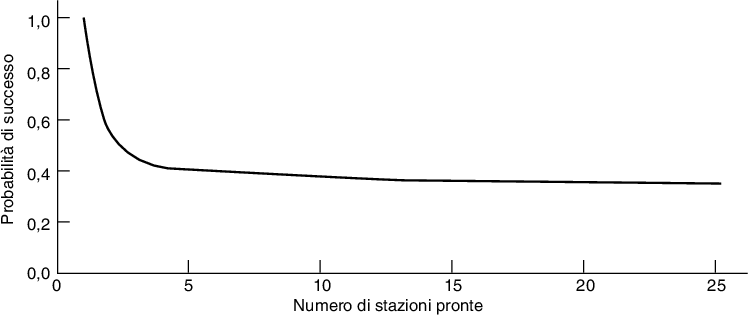
\includegraphics[width=0.6\textwidth]{images/canali_simmetrici.png}
\end{center}
In particolare, se ci sono $N$ stazioni pronte a trasmettere la probabilità che la prima riesca è $n \cdot p \cdot (1-p)^{n-1}$, dove $p$ è la probabilità di trasmettere all'inizio di un certo slot, $1-p$ la probabilità di non farlo. È necessario moltiplicare questa probabilità per $n$, in quanto dobbiamo considerare i casi in cui vinca la seconda, la terza ... l'ennesima, dunque otteniamo $n^2 \cdot p \cdot (1-p)^{n-1}$. La sua derivata con $n$ fissato è $n^2 \cdot (1-p)^{n-1} \cdot (1-\frac{p \cdot n-p}{1-p})$, studiandone il segno ricaviamo che il suo massimo è in $p=\frac{1}{n}$. Dunque al variare degli utenti scegliamo un p opportuno per massimizzare le prestazioni. Ad esempio con 2 utenti è necessario scegliere $p=\frac{1}{2}$.\\
Serve dunque un sistema che riduca la competizione dinamicamente (riduca $p$) al variare degli utenti, nascono quindi i protocolli a contesa limitata.

\subsection{Protocolli a contesa limitata - Adaptive Tree Walk}
L'idea è quella di applicare la tecnica \textit{divide-et-impera} al periodo di contesa.\\
\begin{center}
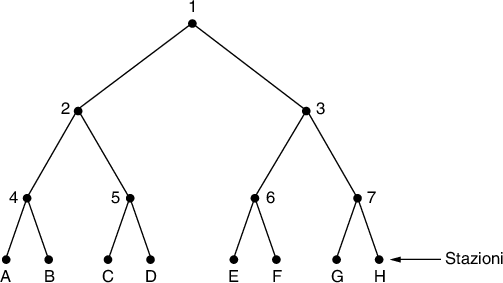
\includegraphics[width=0.4\textwidth]{images/adaptive_tree_walk.png}
\end{center}
Nel primo slot temporale del periodo di contesa tutte le stazioni competono. Se c'è collisione metà di esse vengono silenziate, mentre si ripete ricorsivamente il procedimento con l'altra metà finché qualcuno non si aggiudica un canale oppure resta un solo host attivo. In questo modo il numero di collisioni è logaritmico al numero di utenti.\\
Tuttavia richiede un controllo centralizzato per decidere chi entra in competizione ad ogni turno.\\
Analizzando il traffico di rete, inoltre, è possibile prevedere quante stazioni proveranno a trasmettere e iniziare dal punto dell'albero che si preferisce. È inutile sprecare tempo a partire dalla cima dell'albero se vi sono troppi utenti.\\
Per calcolare l'altezza dell'albero da cui cominciare facciamo questo ragionamento:
\begin{itemize}
\item se siamo in un nodo a profondità $p$ in un albero con $A$ stazioni attive, i nodi sotto di lui sono $A-2^p$
\item se le stazioni attive $A$ sono distribuite equamente (come in figura), allora ci saranno circa $A/2^p$ stazioni attive nel sottoalbero
\item avremo il sottoalbero più piccolo con una sola stazione attiva $\iff A/2^p=1 \iff A=2^p \iff p=log_2A$
\end{itemize}
Quindi la profondità da cui cominciare è data in funzione delle stazioni attive secondo la funzione sopra scritta.

\subsection{Protocolli per LAN wireless}
Nelle reti wireless vi sono ulteriori difficoltà dovute alla topologia della rete che cambia dinamicamente, mentre tutte le tecniche viste fin'ora assumono una topologia fissa in cui gli host non si muovono. Non esiste più quindi un singolo canale, ma varie zone spaziali dette \textit{bolle} dove alcune stazioni interagiscono, altre no.\\
Ogni host è al centro della sua bolla locale, dunque il controllo da globale diventa distribuito e mobile.\\
Sorgono quindi 2 problemi:
\begin{itemize}
\item \textit{Hidden station problem}: è impossibile rilevare con certezza se il canale è libero a causa delle bolle. Ad esempio A trasmette a B, ma C non sente e conclude che il canale è libero, trasmettendo a sua volta. Nella bolla di B c'è collisione.
\item \textit{Exposed station problem}: è possibile che venga rilevata una trasmissione e ci si blocchi, nonostante è possibile trasmettere. Ad esempio B trasmette ad A, C se ne accorge e conclude che non può trasmettere a D, anche se potrebbe visto che non interferisce con A.
\end{itemize}
\begin{center}
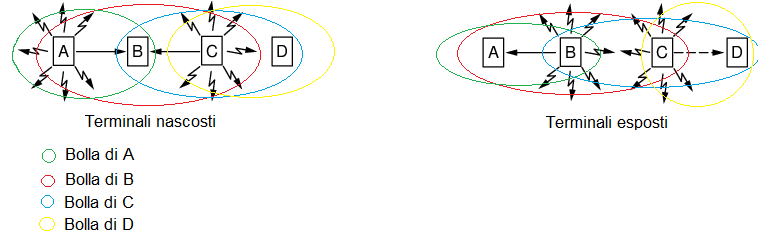
\includegraphics[]{images/problemi_wireless.png}
\end{center}
Di soluzioni a questi problemi ce ne sono varie, analizzeremo solo \textit{MACAW (Multiple Access with Collision Avoidance Wireless)}.
Questo protocollo sfrutta l'idea che chi deve trasmettere renda il suo spazio locale conosciuto anche agli altri. Si fa tramite due comandi:
\begin{itemize}
\item \textit{RTS (Request To Send)}: rende nota la volontà di trasmettere un messaggio ad un certo host nella bolla locale.
\item \textit{CTS (Clear To Send)}: ACK, significa pronto a ricevere.
\end{itemize}
Tuttavia MACAW non è collision free, quando qualcosa va storto si usa ALOHA. In questo modo tutti gli altri utenti nelle bolle del trasmittente e del ricevente sono al corrente della trasmissione in corso e agiranno di conseguenza. Occorre quindi introdurre degli ACK di ricezione RTS da parte di tutti gli host nella bolla. È possibile inoltre inserire la durata della trasmissione all'interno del RTS.

\subsection{Ethernet}
Ethernet è il protocollo predominante allo strato data link nella rete internet. Ne esistono due tipi:
\begin{itemize}
\item \textit{Ethernet classica}: è la forma originale e permette tassi di trasmissione dati dai 3 ai 10 Mbps.
\item \textit{Ethernet commutata (switched)}: è l'evoluzione dell'originale che prevede l'utilizzo di switch (dispositivo di livello data link) anziché hub (dispositivo di livello fisico), raggiungendo velocità di 100, 1000 e 10,000 Mbps.
\end{itemize}
In questi protocolli è stata scelta la \textit{codifica di Manchester} (segnale da alto a basso se 1, da basso a alto se 0) per inviare bit nel canale trasmissivo, in quanto, seppur inefficiente, risulta necessaria quando la rete aumenta di velocità. Con le altre tecniche ci sarebbe un grave problema di perdita di sincronizzazione.

\subsubsection{Tipi di Ethernet}
Nei seguenti tipi di rete il primo numero indica la velocità massima raggiunta espressa in Mbps, base indica che si trasmette in banda base, mentre l'ultimo numero indica il tipo di cavo.
\begin{itemize}
\item \textbf{10 base 5 - thick ethernet} è la primissima versione. Il mezzo trasmissivo è un grosso cavo coassiale con tacche ogni 2.5 metri conficcate nel cavo per permettere l'inserimento dei vari dispositivi. È possibile costruire 5 segmenti di rete senza ripetitore, non superando comunque i 500 metri totali. Ogni segmento può contenere fino a 100 stazioni, la connessione fisica avviene tramite i \textit{vampire taps} (letteralmente morsi di vampiro), che rovinano il cavo.\\
Ad ogni giuntura si trova un \textit{trans receiver}, addetto a carrier detection e collision detection.
\item \textbf{10 base 2 - thin ethernet} è l'evoluzione della precedente che prevede l'uso di un cavo coassiale più fino. Al posto dei pessimi vampire taps si usano delle \textit{giunzioni a T} per l'inserimento dei dispositivi. Il transreceiver si sposta ora dal cavo all'interno dei PC. La lunghezza massima della rete è però ridotta a 200 metri, in cui ogni segmento di rete può tenere fino a 30 stazioni.
\item \textbf{10 base T,} dove T sta per \textit{twisted pair}, di fatto si usano collegamenti in UTP in questa rete, meno costoso e più affidabile dei precedenti. I segmenti di cavo sono però ridotti a 100 metri, tuttavia il numero di stazioni per segmento è aumentato a 1024.
\item \textbf{10 base F} prevede la realizzazione dei segmenti in \textit{fibra ottica}, di conseguenza segmenti lunghi fino a 2 km. Tuttavia vi sono problemi di derivazione, in quanto è difficile inserirsi in un cavo in vetro. Risulta utile per connettere edifici.
\end{itemize}

\subsubsection{Frame Ethernet}
\begin{center}
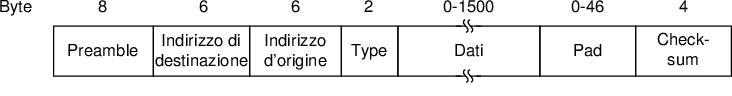
\includegraphics[width=0.7\textwidth]{images/frame_ethernet.png}
\end{center}
\begin{itemize}
\item \textbf{Preambolo:} il primo campo annuncia l'arrivo di un frame ethernet e crea sincronia. È formato da 8 byte (64 bit) formato da 1 e 0 alternati.
%\newpage
\item \textbf{Indirizzo di destinazione:} contiene \textit{l'indirizzo MAC} della destinazione, formato da 6 byte (48 bit) così formato:
\begin{center}
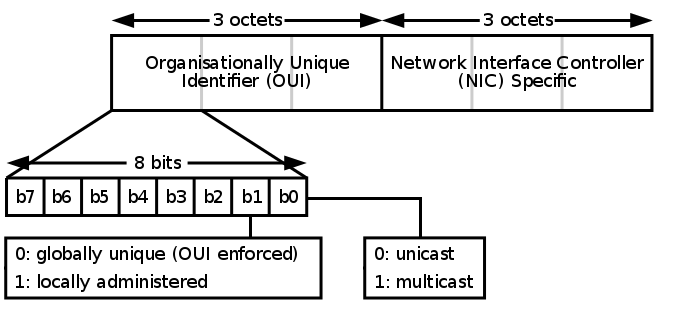
\includegraphics[width=0.5\textwidth]{images/indirizzo_MAC.png}
\end{center}
Il primo bit a 1 segnala una trasmissione multicast (ad un gruppo di host), il secondo indica se è un indirizzo locale o globale gestito da OUI. I primi 3 byte identificano il produttore della scheda di rete, che acquista un gruppo di indirizzi MAC da OUI. I secondi 3 byte servono per l'indirizzamento vero e proprio. Dunque con ogni pacchetto di indirizzi si possono indirizzare $2^{24}$ dispositivi. Esistono $2^{22}$ pacchetti di indirizzi.
\item \textbf{Type:} specifica il tipo di protocollo o la lunghezza del frame.
\item \textbf{Payload:} è il carico pagante e contiene al massimo 1500 byte (solitamente MTU è impostato a questa grandezza).
\item \textbf{Pad:} significa padding, ovvero riempitivo. Serve ad aumentare la lunghezza del frame nel caso sia più piccola della minima consentita. Il parametro di lunghezza minima serve per evitare che una stazione finisca la trasmissione di un frame prima che arrivi a destinazione, in modo da garantire il rilevamento delle collisioni. In generale la lunghezza minima del frame deve garantire che il tempo di trasmissione sia maggiore del tempo di roundtrip. Per ethernet a 10 Mbps il frame deve essere almento 500 bits (512 bits - 64 byte).
\item \textbf{Checksum:} serve per error detection, calcolato con CRC-32.
\end{itemize}

\subsubsection{Backoff esponenziale binario}
In ethernet quando viene rilevata una collisione si usa l'algoritmo CSMA/CD 1-persistente. Tuttavia, per migliorarne le prestazioni, si usa il \textit{binary exponential backoff}: se avviene una collisione il tempo viene diviso in slot, ogni stazione prima di riprovare a trasmettere attende un numero casuale di slot compresi tra 0 e $2^i-1$, dove $i$ è il numero di tentativi. Una volta arrivati a 10 tentativi il valore di $i$ rimane bloccato a 10, permettendo la scelta tra 0 e 1023 slot. Dopo 20 tentativi totali, se la trasmissione non va ancora a buon fine, la scheda di rete rinuncia.

\subsubsection{Efficienza di Ethernet}
L'efficienza media è circa $1/(1+bandwidth \cdot RTD/cF)$, dove $c$ è la velocità di propagazione del segnale e $F$ la lunghezza del frame. Dunque aumentando banda e/o lunghezza diminuiscono le prestazioni, bisogna dunque sacrificare uno dei due fattori. Se aumentiamo la banda bisogna diminuire la lunghezza massima dei collegamenti di rete e viceversa.\\
Per sopperire a questo problema si sostituiscono gli hub con gli switch.
\paragraph{HUB} È l'equivalente di una connessione fisica, ovvero propaga il segnale in ingresso su una porta in tutte le uscite (compresa quella d'ingresso). È un dispositivo economico, poco complesso e affidabile, tuttavia non risolve il problema dei limiti della rete e non può connettere reti eterogenee.
\paragraph{SWITCH - BRIDGE} Sono essenzialmente lo stesso dispositivo, solamente con la differenza che gli switch sono usati in reti più piccole, i bridge in reti grandi. La loro peculiarità è quella di interagire con la struttura del frame, sono quindi dispositivi di secondo livello (data link). Vengono quindi usati per unire due o più reti anche eterogenee, tenendole per quanto possibile distinte per evitare problemi derivati dalla eccessiva grandezza di reti singole. Si crea quindi una rete più grande solo a livello logico, non fisico, creando diversi domini di collisione.\\
Questo effetto si ottiene ispezionando i frame e analizzando il traffico. Serve una fase iniziale in cui lo switch impara la configurazione di rete:
\begin{itemize}
\item Controlla mittente e destinatario dei frame (MAC address).
\item Effettua il \textit{backward learning}, costruendo hash table tramite l'analisi del flusso dati e relative risposte, utilizzando la trasmissione broadcast.
\item Si introduce il concetto di \textit{information fading}, ovvero c'è un timeout che causa la scadenza di un'informazione se non viene refreshata da frame di passaggio.
\end{itemize}
Sorge ora il problema dei \textit{loops} all'interno delle reti, poiché i frame potrebbero continuare a girare per questi pezzi di rete all'infinito. È necessario trasformare il grafo che rappresenta la topologia di rete in un albero, che per definizione non ha cicli. Questo procedimento si chiama \textit{calcolo dello spanning tree}. Gli switch disattivano alcune porte seguendo il protocollo 802.1D, che mette in comunicazione tutti gli switch dando una visione globale della topologia. Si segue questo algoritmo:
\begin{itemize}
\item Inizialmente si elegge il nodo root, in base a chi ha il MAC address minore.
\item Viene quindi costruito un albero con i percorsi più brevi dalla radice ad ogni nodo.
\item Per trovare questi percorsi minimi i bridge includono la loro distanza dalla radice nei messaggi di configurazione. Ogni bridge ricorda il percorso più breve verso la radice e spengono le porte che non coinvolgono questo tragitto.
\item L'algoritmo continua ad essere eseguito durante il normale funzionamento della rete per rilevare cambi di topologia e aggiornare l'albero.
\end{itemize}
Tuttavia resta il problema dei \textit{colli di bottiglia} che si creano quando si collegano reti veloci con reti lente oppure i flussi sono sbilanciati. Aggiungere memoria buffer agli switch peggiora la cosa, poiché viene inoltrata informazione scaduta. Si passa quindi l'onere al livello superiore di rete.

\subsubsection{Evoluzione di Ethernet}
Col passare del tempo, la velocità massima di 10 Mbps offerta da ethernet classica divenne troppo limitativa. Nacque quindi \textit{Ethernet commutata}, che faceva uso degli switch prima descritti.
\paragraph{Fast Ethernet} Si decise di mantenere le caratteristiche native di ethernet, mantenendo quindi i suoi problemi, aumentando la velocità a 100 Mbps, rendendola quindi retrocompatibile. La soluzione alternativa, che prevedeva di ricostruire da capo il protocollo, fallì miseramente per la mancanza di questa caratteristica anche se migliore in teoria, poiché eliminava tutti i problemi iniziali.\\
Venne quindi semplicemente incrementato il clock di un fattore 10, con conseguenti limitazioni della lunghezza della rete. A questo proposito vengono introdotti gli switch. Ci sono diversi tipi di Fast Ethernet:
\begin{itemize}
\item 100 base T4: collegamenti composti da 4 cavi UTP 3, permettendo una lunghezza massima della rete di 100 metri.
\item 100 base TX: collegamenti composti da un cavo UTP 5, è anche la versione di ethernet più in voga. La lunghezza massima è ancora 100 metri.
\item 100 base FX: collegamenti in fibra ottica, la lunghezza massima della rete è ora 2 km.
\end{itemize}
\paragraph{Gigabit Ethernet} Il fattore di velocità del clock viene moltiplicato ancora una volta di 10 rispetto a fast ethernet, raggiungendo di fatto la velocità di 1 Gbps (1000 Mbps). Viene rimosso il carrier sense per aumentare di molto la velocità, tuttavia la lunghezza del cavo cala drasticamente. Per risolvere questo problema è possibile aumentare la dimensione dei frame aggiungendo padding (soluzione pessima e inefficiente), oppure spedire i frame a blocchi (\textit{frame bursting}), riportando la lunghezza massima a 200 metri.\\
In questa versione di Ethernet è necessario che gli switch siano velocissimi nelle operazioni di forward, poiché per un ritardo di un millisecondo vengono persi circa 2000 frame. In caso di rallentamento dello switch viene introdotto un frame speciale per mettere in pausa la trasmissione.

\subsection{Standard wireless 802.11}
Posiziona le trasmissioni negli spettri dei 2.4 Ghz e 5 Ghz, compresi nelle frequenze libere. C'è quindi un problema di interferenza con altri dispositivi che fanno uso dello stesso spettro (es. forni a microonde). Esistono varie versioni del protocollo, scritte in ordine temporale.
\begin{itemize}
\item 802.11b con data rate fino a 11 Mbps, utilizzando HR-DSSS, ovvero modulazione di fase con trasmissioni 7 volte più estese di 802.11a utilizzando codici di Walsh-Hadamard.
\item 802.11a con data rate fino a 54 Mbps lordi, utilizzando QAM e OFDM nella banda a 5 Ghz
\item 802.11g che riporta il data rate a 54 Mbps, utilizzando ancora OFDM ma nella banda ristretta dei 2.4 Ghz
\item 802.11n che introduce \textit{MIMO} (Multiple Input - Multiple Output) usando 4 \textit{smart antennas}, ovvero antenne direzionali. Si arriva a 600 Mbps di banda, usando canali da 40 Mhz rispetto ai 20 Mhz dei precedenti, oppure passa alla banda dei 5 Ghz, diminuendo il raggio d'azione ma aumentando il numero di dispositivi che si possono connettere. Usa una codifica QAM-64.
\item 802.11ac porta il data rate ad un massimo di 860 Mbps, usa la banda dei 5 Ghz e canali da 160 Mhz usando 8 antenne direzionali e QAM-256.
\end{itemize}
Lo standard prevede due diversi modi operativi:
\begin{itemize}
\item \textbf{DCF} (Distributed Coordination Function) prevede un controllo distribuito, utilizzando CSMA/CA (evita le collisioni) in due diverse tipologie:
	\begin{itemize}
	\item CSMA/CD non persistente con truncated binary exponential backoff
	\item MACAW con frame RTS e CTS includendo in questi la durata della trasmissione.
	\end{itemize}
\item \textbf{PCF} (Point Coordination Function) in cui il controllo è centralizzato. La stazione controllore invia frame "beacon" con i comandi per le altre stazioni.
\end{itemize}
Le due metodologie possono coesistere, tuttavia i comandi PCF hanno la priorità.\\\\
802.11 offre i seguenti \textbf{servizi}: connessione (association), chiusura connessione (disassociation), cambio stazione di base (reassociation), modalità di invio frame alla stazione base (distribution), traduzione in altri formati (integration).\\\\
Le \textbf{interferenze nella rete wireless} possono provenire dall'ambiente circostante o da altre reti wireless, anche con protocolli diversi. Esistono 3 soluzioni a questo problema:
\begin{enumerate}
\item \textit{CTS protection mode} (disattivata di default) attiva la modalità MACAW. Provoca un overhead ma riduce il numero di collisioni. Tutte le reti prevedono un CTS threshold, ovvero la soglia di tolleranza sopra la quale si attiva questa protezione.
\item \textit{Fragmentation threshold} è la soglia massima per la taglia dei pacchetti in arrivo dal livello superiore. Se superano questa soglia vengono frammentati. Protezione utile quando MACAW fallisce. Le performance decadono rapidamente quando attivata, perciò si applica il frame burst e sliding window in simultanea.
\item \textit{Cambiare frequenza} quando i precedenti due metodi falliscono. Questo causa la disconnessione di tutti i dispositivi attualmente connessi. 802.11 sulla frequenza dei 2.4 Ghz prevede 13 canali diversi.
\end{enumerate}

\subsection{Bluetooth}
\begin{minipage}{0.55\textwidth}
Protocollo per reti micro locali (low range). Il requisito fondamentale è il basso consumo di energia, poiché usato in dispositivi mobili. Si formano delle pico-net, con al centro il nodo master, gli altri sono nodi slave, a loro volta active o parked (sospeso). Possono esserci al massimo 7 nodi slave attivi. Per unire più pico-net si nomina uno slave bridge, creando le scatternet.\\Un problema che sorge è l'interferenza con le reti Wi-Fi.
\end{minipage}
\begin{minipage}{0.45\textwidth}
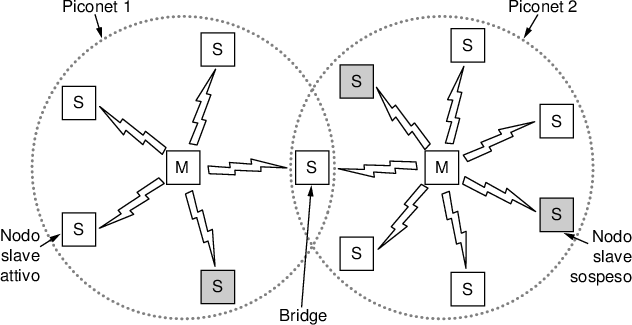
\includegraphics[width=\textwidth]{images/pico_net.png}
\end{minipage}
Il \textbf{frame bluetooth} è così composto:
\begin{center}
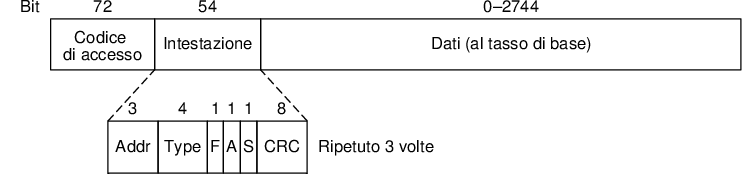
\includegraphics[width=0.7\textwidth]{images/frame_bluetooth.png}
\end{center}
\begin{itemize}
\item \textit{L'Access code} è l'ID del nodo master, gli schiavi ascoltano solo il nodo master con un certo ID.
\item \textit{Data} è il classico payload di lunghezza variabile.
\item \textit{L'Header} è a sua volta composto da:
	\begin{itemize}
	\item Addr: indirizzo dello slave attivo
	\item Type: tipo di frame, lunghezza del frame, sistema di error correction. Esistono due tipi di frame:
		\begin{itemize}
		\item ACL: Asyncronous Connection-Less (senza canale)
		\item SCO: Syncronous Connection-Oriented (con canale)
		\end{itemize}
	\item F: Flow, interrompi trasmissione, buffer pieno
	\item A: ACK
	\item S: Sequence, controllo di flusso stop-and-wait
	\item Checksum: rilevamento errori con CRC
	\end{itemize}
Il campo header viene ripetuto 3 volte per evitare errori.
\end{itemize}

\section{Livello di rete}
Il livello di rete si occupa del trasporto dei pacchetti lungo tutto il percorso dall'origine alla destinazione finale. Deve perciò conoscere la topologia della rete di comunicazione e scegliere i percorsi appropriati.\\
Inoltre si occupa di gestire il traffico di rete in modo da evitare le congestioni e garantire la qualità del servizio.

\subsection{Algoritmi di routing}
Il routing è un processo in cui si decide la via che deve seguire un pacchetto per andare da un punto A ad un punto B nella rete.
La scelta più comune è quella di minimizzare il numero di \textit{hops} lungo il cammino, ovvero le stazioni di terzo livello (router) attraversate. Tuttavia non è sempre la soluzione vincente.\\
 Nel \textit{routing non adattivo} (applicato nella rete telefonica) vengono calcolate le distanze minime nel grafo con l'algoritmo di Dijkstra. Ogni nodo avrà quindi una tabella che gli indica dove mandare i pacchetti a seconda della destinazione indicata solitamente nell'header del protocollo di rete.\\
Nel \textit{routing adattivo} la rete subisce molte variazioni, sia fisiche che di flusso. Per conoscere la topologia di rete viene usato il \textbf{flooding} (inondazione), ovvero la Nutella delle reti (mangiarne poca altrimenti si sta male, anche se è buona).

\subsubsection{Flooding}
Con questa tecnica ogni pacchetto viene ritrasmesso a tutte le linee esclusa quella d'ingresso in broadcast. La rete viene sommersa da pacchetti ridondanti. Tuttavia funziona con tutti i tipi di trasmissione (point-to-point, multicast e broadcast), sceglie sempre la via migliore (le sceglie tutte) ed è robusto rispetto alle modifiche di rete (funziona sempre).\\
Per arginare l'alluvione vengono adottate delle tecniche di \textbf{controllo del flooding}:
	\begin{itemize}
	\item \textit{Hop counting}: inserimento di un valore TTL (Time To Live) che viene decrementato ogni volta che il pacchetto viene inoltrato. Se si riceve un pacchetto con TTL=0 viene scartato.
	\item \textit{Tracking}: si tiene traccia dei pacchetti già inoltrati. Servirebbe un buffer enorme, perciò si tiene solamente il numero di pacchetti inoltrati, tutti i pacchetti con numero di sequenza minore vengono scartati.
	\end{itemize}
	Il flooding è l'unico algoritmo di routing che trova sempre la via migliore, anche al variare della rete. È utile quando il carico di rete è basso ma la topologia è estremamente variabile o i messaggi sono critici, nasce infatti in ambito militare.

\subsubsection{Distance vector routing}
Un protocollo meno estremo del flooding è quello basato sul \textit{vettore delle distanze}, chiamato anche algoritmo di Bellman-Ford e tutt'ora in uso su Internet con il nome di RIP.\\
Qui ogni router ha una tabella di routing che contiene informazioni su quanto veloce è la connessione per un certo collegamento. Questa tabella è formata chiedendo ai vicini la propria e integrando i nostri dati, ottenuti tramite pacchetti ECHO inviati alle stazioni vicine.
La tabella contiene il next hop e la distanza per raggiungere un certo nodo, calcolata con l'algoritmo di Dijkstra. Ecco un esempio del processo di aggiornamento delle tabelle che avviene periodicamente.
\begin{center}
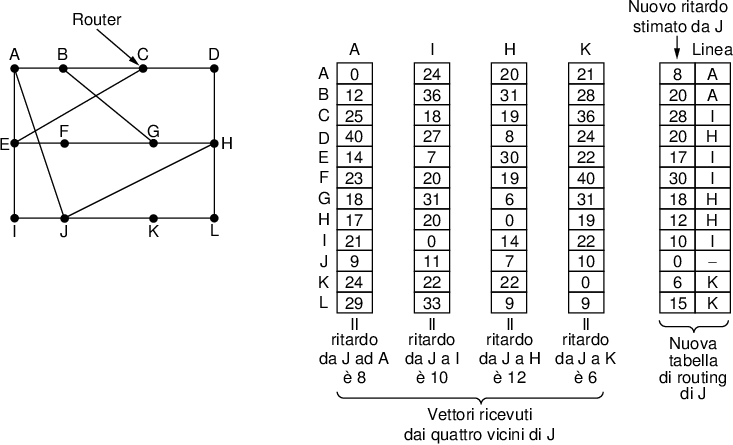
\includegraphics[width=0.6\textwidth]{images/distance_vector_routing.png}
\end{center}
Vediamo come viene creata la tabella del router $J$. Le prime 4 tabelle sono i vettori di ritardo ricevuti dai suoi vicini. Ad esempio $A$ dichiara un ritardo di 12 millisecondi verso B, di 25 ms verso C, etc... Si supponga che $J$ abbia misurato i ritardi verso i suoi vicini $A, I, H, K$ rispettivamente pari a 8, 10, 12 e 6 ms. Poiché $J$ sa di poter raggiungere $A$ in 8 ms e $A$ dichiara di poter arrivare a $G$ in 18 ms, sa che trasmettendo i suoi pacchetti verso $A$ potrà raggiungere $G$ in 26 ms. In modo analogo la distanza da $G$ viene calcolata passando attraverso gli altri vicini. Il valore migliore è 18 ms e si ottiene passando per $H$, si registra quindi questo risultato. Lo stesso calcolo è eseguito per tutte le destinazioni.\\\\
Questo algoritmo riconosce molto bene i cambiamenti positivi della rete, tuttavia è molto lento nel riconoscere quelli negativi. Il processo di assestamento dei percorsi verso la configurazione dei cammini ottimi è chiamato \textbf{convergenza}.\\
Sorge il problema del \textbf{conteggio all'infinito}, in cui questo processo tende a divergere in caso di peggioramento della rete.\\\\
\begin{minipage}{0.3\textwidth}
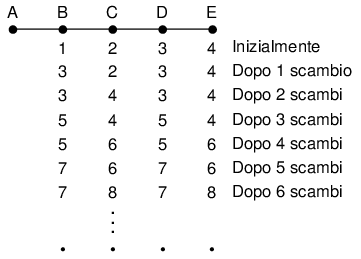
\includegraphics[width=\textwidth]{images/count_to_infinity.png}
\end{minipage}
\begin{minipage}{0.7\textwidth}
Consideriamo la topologia di rete in figura, in cui $A$ esce dalla rete. Al primo scambio di pacchetti $B$ non riceve nulla da $A$. Di conseguenza pensa di poter raggiungere $A$ attraverso $C$ poiché non può sapere che il percorso da $C$ ad $A$ comprende lui stesso. Al secondo scambio $C$ si accorge di non comunicare con $A$, decidendo quindi di dirottare il traffico verso quella stazione attraverso $D$, che dichiara di avere una linea funzionante per $A$.\\
In linea di massima nessun router ha mai un valore che supera di oltre un'unità quello minimo di tutti i vicini. Lentamente tutti i router trovano la strada per l'infinito, che dipende dal valore numerico usato per rappresentarlo. Solo una volta che viene raggiunto tale valore una destinazione viene dichiarata irraggiungibile ed esclusa dalle tabelle di tutti.
\end{minipage}

\subsubsection{Link state routing}
Un'alternativa agli algoritmi precedenti è il routing basato sullo \textit{stato dei collegamenti}.\\
Si costruisce inizialmente una tabella locale con le distanze verso tutti i vicini calcolate inviando il pacchetto HELLO e misurando il tempo di risposta. L'informazione locale viene poi mandata in broadcast sulla rete con il flooding, che viene eseguito periodicamente per fare il refresh dell'informazione, poiché si usa \textit{l'information fading}. Questa tecnica spreca più banda ma è molto più robusta alle variazioni della rete.\\
Se la rete è troppo grande il flooding crea problemi (troppa Nutella non fa bene), perciò si usa il \textit{reverse path forwarding}, una variante del flooding in cui vengono inoltrati solo i pacchetti provenienti dal cammino migliore, ipotizzando che tutti gli altri siano cloni.

\subsubsection{Routing gerarchico}
\begin{minipage}{0.7\textwidth}
Per limitare gli effetti devastanti del flooding è possibile dare una struttura gerarchica alla rete, dividendo i router per regioni.\\
Invece di inondare tutta la rete lo facciamo solo su una regione. Ogni router conosce i dettagli solo della sua regione, mentre sa solamente come arrivare ad una regione esterna alla sua ma non la topologia.\\
Il prezzo da pagare è l'incremento della lunghezza di determinati percorsi, poiché non è più possibile trovare il cammino minimo in assoluto.\\
Il numero ottimale di livelli gerarchici per una rete composta da $N$ router è $ln(N)$, per un totale di $e\cdot ln(N)$ voci per router.
Inoltre l'aumento della lunghezza del percorso medio causato da questo algoritmo è sufficientemente piccolo da renderlo accettabile.
\end{minipage}
\begin{minipage}{0.3\textwidth}
\begin{flushright}
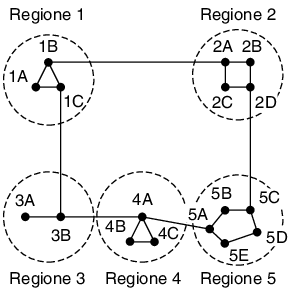
\includegraphics[width=0.85\textwidth]{images/routing_gerarchico.png}
\end{flushright}
\end{minipage}

\subsection{Quality of Service - QoS}
Alcune applicazioni richiedono garanzie di prestazioni. Ad esempio le applicazioni multimediali richiedono alla rete una capacità minima e un ritardo massimo.\\
Le esigenze di ogni flusso possono essere riassunte in 4 parametri:
\begin{itemize}
\item \textit{Affidabilità:} certezza di consegna di tutti i pacchetti
\item \textit{Ritardo:} i pacchetti devono essere consegnati entro un certo tempo limite (ping)
\item \textit{Jitter:} limite di oscillazione di rete, influenza l'ordine di arrivo dei pacchetti
\item \textit{Banda:} serve un data rate minimo di trasmissione
\end{itemize}
Questi parametri caratterizzano la qualità del servizio richiesta da un determinato flusso.

\subsection{Algoritmi per il controllo della congestione}
Come gestire le congestioni non è affatto ovvio poiché certe azioni portano ad effetti paradossali. L'andamento delle performance di una rete vittima di congestione è rappresentato nel grafico seguente.
\begin{center}
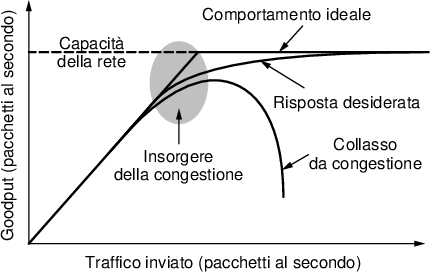
\includegraphics[width=0.4\textwidth]{images/congestione.png}
\end{center}
Ad esempio aggiungere capacità ad una rete (aumentando la banda o aggiungendo nuovi collegamenti) può portare ad una diminuzione delle performance. Questo perché si è incastrati nel minimo dell'\textit{equilibrio di Nash} visto che facciamo tutti la stessa scelta. Queste situazioni si superano con un controllo centralizzato, togliendo la capacità di scelta dei singoli router. In questo modo le scelte saranno benefiche per tutto il gruppo, non solo per il singolo individuo. Lasciando il controllo distribuito ognuno fa scelte vantaggiose solo per se stesso, senza pensare alla collettività.\\\\
Per le reti \textbf{virtual circuit} (a circuito virtuale) è semplice centralizzare il controllo. Qui la rete è orientata alla connessione, si può quindi effettuare \textit{admission control}, ovvero si può proibire la creazione di nuovi canali. Si può inoltre dirottare il traffico (\textit{traffic aware routing}) se sta andando verso nodi congestionati modificando il canale, tuttavia con si crea l'effetto see-saw (altalena), in cui aumenta il jitter (indice di oscillazione della rete). In questo tipo di gestione c'è un grande spreco di banda a causa dell'allocazione statica del canale.\\\\
Per le reti \textbf{datagram}, ovvero senza connessione, la rete è dinamica ed è necessario evitare lo spreco di banda e tempo. Qui il controllo centralizzato è impraticabile. Non è nemmeno possibile potenziare singoli nodi ad esempio aumentando il buffer, in quanto la rete collassa per l'effetto valanga provocato dall'inoltro d'informazione scaduta.\\
Analizziamo le varie possibilità di controllo del traffico in questo tipo di reti.

\subsubsection{Choke packet}
Il ricevente può manifestare la congestione soffocando il mittente inviandogli il \textit{choke packet}. Chi riceve questo pacchetto deve dimezzare il data rate di trasmissione. Se chi invia troppi pacchetti stava solo ritrasmettendo allora semplicemente inoltra il choke al reale trasmettitore. Viene anche qui usato il fading, ovvero se il mittente non riceve altri choke rialza gradualmente il data rate. Inoltre, non appena si riceve un choke, per un determinato periodo di tempo successivo non considero altri choke in quanto potrebbero essere cloni generati dalla rete.\\\\
Se la rete è grande una richiesta di choke potrebbe metterci troppo tempo ad essere accolta, si introduce perciò il \textbf{choke packet hop-by-hop}, che strozza tutti i router che coinvolgono il tratto dal mittente al destinatario che si sta congestionando, ottenendo un beneficio immediato.

\subsubsection{*Notifica esplicita di conversione}
Invece di generare pacchetti specifici per la notifica di congestione un router può etichettare i pacchetti che inoltra per segnalare che c'è una congestione in atto (piggyback). Questo metodo è chiamato \textit{ECN}. Se uno qualsiasi dei router attraversati dal pacchetto è congestionato gli viene attaccato in piggyback la notifica di congestione.

\subsubsection{Load shedding}
Questa tecnica deriva dalla rete elettrica, nella quale in caso di congestione si butta via il carico. Analogamente nelle reti di calcolatori alcuni pacchetti vengono scartati. È una scelta estrema ma ragionevole, in quanto piuttosto che rallentare tutta la rete penalizzo il ricevente, al quale non arriveranno pacchetti, tanto la rete ha già le dovute protezioni per evitare perdite e richiedere ritrasmissioni (ACK etc...). È possibile affinare la tecnica scegliendo i pacchetti da scartare:
\begin{itemize}
\item \textbf{Wine:} il vino più invecchia e più è buono. Analogamente i pacchetti più recenti vengono scartati, preservando quelli vecchi. Utile in canali che trasportano dati di login o file.
\item \textbf{Milk:} il latte, al contrario, è meglio fresco piuttosto che vecchio. Analogamente vengono scartati prima i pacchetti più vecchi. Usato su applicazioni di streaming e sistemi real-time, dove conta andare veloce a scapito della qualità.
\end{itemize}
È possibile migliorare questa tecnica con il buffering, il quale non risolve la congestione ma riduce il jitter. Usato spesso nei servizi di streaming video online.

\subsubsection{*RED - Random Early Detection}
Risulta più semplice gestire la congestione appena viene rilevata piuttosto che cercare di porvi rimedio dopo che tutto si ferma. I chocke packet o i pacchetti con ECN potrebbero non arrivare a destinazione a causa della congestione e del possibile load shedding. L'unico modo affidabile per riconoscere una congestione è quando i router iniziano a scartare pacchetti. Facendo in modo che ciò accada prima che la situazione diventi disastrosa è possibile bloccare il problema sul nascere.\\
Quando la lunghezza delle code di pacchetti nel buffer diventa più lunga della norma scatta questa protezione; i router iniziano a fare load shedding anche se la memoria non è piena.\\
ECN resta comunque una tecnica preferibile a RED in quanto evita la perdita, tuttavia RED è necessaria quando gli host non possono ricevere segnali espliciti.

\subsubsection{Traffic shaping}
Consiste nell'accordare mittente e destinatario sul rate di trasmissione da mantenere (\textit{Service Level Agreement - SLA}).
L'obiettivo è quello di permettere alle applicazioni di trasmmettere una grande varietà di traffico adatto alle loro necessità, definite dal QoS, inclusi i picchi.\\
Fintanto che il cliente si attiene alla sua parte di accordo e invia pacchetti secondo il contratto concordato, il fornitore promette di consegnare tutti i dati in modo tempestivo.

\subsubsection{Leaky bucket}
\begin{minipage}{0.75\textwidth}
È un filtro (\textit{secchio bucato}) che serve a garantire la QoS. Normalizza il flusso rendendolo costante (limitato). Evita i burst e viene implementato come una coda FIFO. Potrebbe esserci uno spreco di banda, in caso di picchi c'è uno spreco di pacchetti che vengono scartati quando il secchio è piento.
\end{minipage}
\begin{minipage}{0.25\textwidth}
\begin{center}
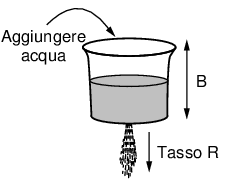
\includegraphics[width=0.6\textwidth]{images/leaky_bucket.png}
\end{center}
\end{minipage}

\subsubsection{Token bucket}
\begin{minipage}{0.75\textwidth}
È l'evoluzione del precedente che risolve il problema dello spreco di banda e di pacchetti in caso di picco. I pacchetti escono solo se ci sono \textit{token} disponibili, i quali si ricaricano quando non c'è nulla da trasmettere e si accumulano. A lungo termine la media del data-rate è costante. Il sistema di token è implementato tramite un semplice contatore. Token e leaky bucket possono essere combinati all'interno della stessa rete.
\end{minipage}
\begin{minipage}{0.25\textwidth}
\begin{center}
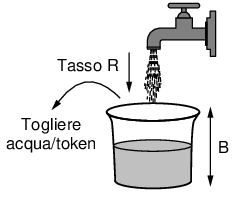
\includegraphics[width=0.6\textwidth]{images/token_bucket.png}
\end{center}
\end{minipage}

\subsection{IP - Strato di rete in Internet}
IP sta per \textit{Internet Protocol}, ed è il protocollo predominante nello strato di rete di Internet.\\
Inizialmente ARPANET usava NCP, che faceva uso di tutte le cose viste fin'ora allo strato di rete. Tuttavia era inadatto alle esigenze del dipartimento della difesa (DoD) degli USA, il quale ha finanziato lo sviluppo di questo protocollo. Le loro richieste erano l'affidabilità e la velocità di consegna, in quanto doveva essere usato in sistemi critici in cui la rete può subire cambi a livello fisico (pezzi di rete saltano in aria in zona di guerra) e il traffico è life critical. Tutte le belle cose viste fin'ora vengono quindi portate in TCP e collocate al livello superiore di trasporto, spezzando il protocollo in TCP/IP. IP deve solamente garantire le funzioni fondamentali, provocando il minimo overhead, dunque deve fornire un servizio non orientato alla connessione e che preferisca effettuare ritrasmissione piuttosto che sprecare tempo in correzione dell'errore.\\
In pratica un protocollo progettato per un ambiente closed-world è stato usato in un ambiente open-world e sbam! copà, mille problemi di sicurezza.

\newpage
\subsubsection{IPv4}
\textbf{HEADER}
\begin{center}
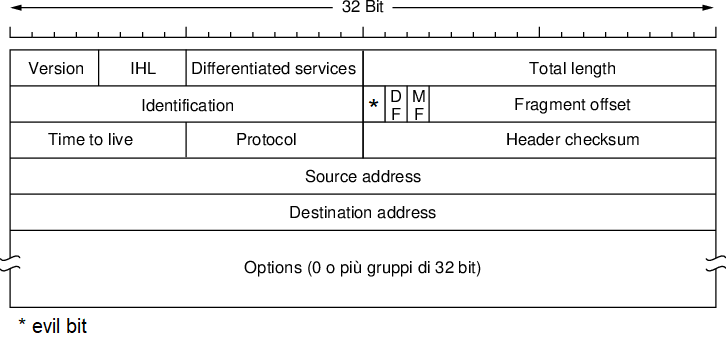
\includegraphics[width=0.6\textwidth]{images/header_ipv4.png}
\end{center}
È composto da una parte fissa di 20 byte (info) e da una seconda parte di lunghezza variabile (options).
\begin{itemize}
\item \textit{Version}: indica la versione di IP in uso (4 in questo caso - 0100).
\item \textit{IHL}: IP Header Length indica la lunghezza dell'header, visto che è variabile.
\item \textit{TOS}: Type Of Service, usato per la QoS (differentiated services)
\item \textit{Total length}: lunghezza di tutto il pacchetto IP.
\item \textit{Identification}: in caso di frammentazione del pacchetto si usa questo campo. Tutti i frammenti derivati dallo stesso pacchetto spezzato hanno questo campo uguale.
\item \textit{DF}: Don't fragment.
\item \textit{MF}: More Fragment, indica se seguiranno altri pacchetti che devono essere ricomposti con questo.
\item \textit{Fragment offset}: numerazione del pacchetto interna alla frammentazione, necessario per ricostruire il pacchetto originale.
\item \textit{Evil bit}: accendo il bit se il contenuto che inserisco nel payload è malevolo :) ottima misura di sicurezza.
\item \textit{TTL:} Time-To-Live indica quante stazioni può ancora attraversare quel pacchetto. Inizializzato solitamente a 255, viene decrementato ogni volta che attraversa una stazione fino a 0, quando viene scartato.
\item \textit{Protocol}: Indica il protocollo allo strato superiore che sta usando IP (TCP, UDP, etc...).
\item \textit{Checksum}: Calcolato tramite somme dell'header in complemento a uno (metodo più sfigato di tutti ma il più veloce).
\item \textit{Indirizzo IP sorgente}
\item \textit{Indirizzo IP destinazione}
\end{itemize}
Per come è strutturato l'header, IPv4 ha dei \textbf{limiti di estendibilità}. IHL è di 4 bit, perciò la lunghezza massima in assoluto è di 60 bytes. Il numero massimo che contiene TTL è 255.\\
Gli indirizzi sono a 32 bit e si stanno esaurendo.\\\\
Sono gestiti da un'autorità centralizzata che li assegna a blocchi di taglia variabile. Esistono diverse classi di blocchi, le principali sono:
\begin{itemize}
\item \textit{Classe A}: 8 bits per la rete, 24 bits per gli host
\item \textit{Classe B}: 16 bits per la rete e 16 per gli host
\item \textit{Classe C}: 24 bits per la rete, 8 per gli host
\end{itemize}
Tecnicamente questa era un'ottima soluzione, tuttavia non teneva conto del fattore psicologico degli utenti. La maggioranza delle persone ha chiesto una classe B quando gli bastava una C per paura di non starci, sprecando di fatto indirizzi.\\
MAC non ha questo problema perché ha una taglia unica, dunque nelle persone non si crea questo effetto psicologico.\\
La soluzione a questo problema esiste da un pezzo e si chiama IPv6. Tuttavia è applicata in pochissimi pezzi di internet.\\
Nel frattempo si è preferito adottare delle soluzioni "tampone", ovvero mettere pezze qua e là, eccone 2.

\subsubsection{CIDR}
\textit{Classless Interdomain Routing} trascende dal concetto di classe di indirizzo IP creando blocchi di lunghezza variabile (potenza del 2). Permette ai router una gestione abbastanza efficiente usando le cosiddette \textit{aggregate entries}, ovvero se ci sono varie classi di indirizzi che devono essere indirizzati allo stesso router, possono essere combinate in un'unica entrata se hanno un prefisso comune.\\
Ad esempio un router riconosce che il next hop per gli indirizzi di rete 194.24.0.0 e 194.24.16.0 è lo stesso.\\
194.24.000|00000.0\\
194.24.000|10000.0\\
hanno lo stesso prefisso, dunque vengono aggregate in un'unica entrata 194.24.0.0.\\
Se c'è un indirizzo con lo stesso prefisso ma destinato ad un altro next hop si usa la regola del \textit{longest matching}, cioè l'entrata con il prefisso di rete che combacia meglio viene scelta. Ad esempio: 194.24.1.0 è compreso tra i due indirizzi prima scritti.\\
194.24.000|00001.0\\
Creo dunque una regola diversa specifica per questo indirizzo.

\subsubsection{NAT}
\textit{Network Address Translation} è il vero salvatore dal disastro creato con la carenza di indirizzi in IPv4.\\
Con questo protocollo si simula un'intera sottorete con un solo indirizzo IP. All'interno la rete ha degli IP locali privati, invisibili all'esterno. Da fuori si vede solamente l'IP pubblico assegnato dall'ISP. Ogni pacchetto che esce dalla rete viene nattato dal dispositivo addetto (solitamente il router), ovvero viene sostituito l'indirizzo mittente privato con quello pubblico. Il problema sorge con i pacchetti in entrata. Questi ultimi arrivano con all'interno l'IP pubblico, dobbiamo quindi capire chi è il vero destinatario. Per farlo è stata fatta l'ennesima porcata: si guarda dentro il payload del livello di trasporto la porta, concetto inesistente allo strato di rete, ricostruendo quindi l'indirizzo IP privato.\\
Per gli indirizzi privati sono stati riservati 10.0.0.0 per le classi A, 172.16.0.0 per le B, 192.168.0.0 per le C.

\subsubsection{ICMP}
\textit{Internet Control Message Protocol} gestisce gli interventi inaspettati, ad esempio se un pacchetto raggiunge TTL=0. Serve per inviare i choke packet e viene incapsulato in IP.\\
Si usa inoltre per effettuare il trace route modificando il valore del campo TTL.

\subsubsection{DHCP}
\textit{Dynamic Host Configuration Protocol} serve per convertire indirizzi MAC in indirizzi IP. Appena una macchina viene inserita in una rete manda un pacchetto di DHCP DISCOVERY, in cui inserisce il suo indirizzo MAC richiedendo un indirizzo IP. Il gestore DHCP (solitamente il router) centralizzato risponde con un IP libero che gli assegna.

\subsubsection{ARP}
\textit{Address Resolution Protocol} serve per convertire indirizzi IP in indirizzi MAC. Questi ultimi sono già assegnati come visto in precedenza, perciò la soluzione è diametralmente opposta al DHCP, distribuita. La richiesta ARP viene inviata periodicamente in broadcast creando una tabella locale delle corrispondenze, che verrà allegata alla prossima richiesta.\\
\textit{ARP request}: una macchina vuole inviare un pacchetto ad un'altra con indirizzo IP X noto, dunque chiedo chi ha l'indirizzo X. Teoricamente chi ha quel IP risponde con la sua ARP table in piggyback.\\
Inoltre quando una macchina si connette ad una rete, dopo aver inviato la DHCP REQUEST, chiede chi ha il suo indirizzo IP e risponde in modo che tutti sappiano. In questo modo ci si accorge anche di IP duplicati nella stessa rete ritornando un errore ad entrambi.

\subsubsection{IPv6}
\begin{minipage}{0.5\textwidth}
La differenza fondamentale con IPv4 è la lunghezza degli indirizzi, ora a 16 bytes invece che 4. Sono ancora a dimensione fissa, tuttavia il numero di indirizzi è troppo grande perché finiscano ($2^{128}=3.4\cdot 10^{38}$). Inoltre è stato rimosso il checksum per velocizzare ancora di più le operazioni di indirizzamento, visto che i canali di trasmissione odierni sono abbastanza affidabili.
\end{minipage}
\begin{minipage}{0.5\textwidth}
\textbf{HEADER}
\begin{flushright}
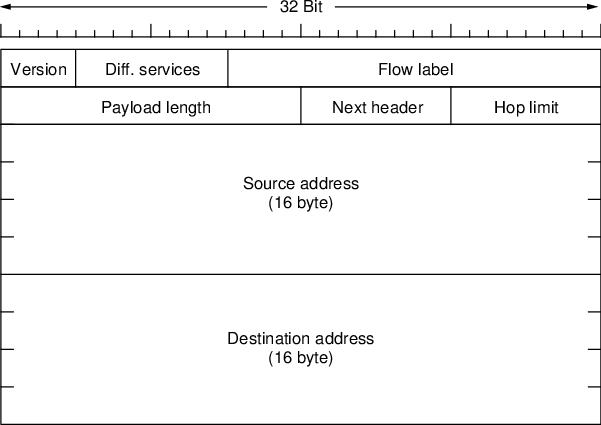
\includegraphics[width=0.9\textwidth]{images/header_ipv6.png}
\end{flushright}
\end{minipage}
\begin{itemize}
\item \textit{Version}: fissa a 6 (0110)
\item \textit{Type of service}: QoS
\item \textit{Flow label}: marca un gruppo di pacchetti che hanno gli stessi requisiti e devono quindi essere trattati allo stesso modo
\item \textit{Payload length}: indica il numero di byte che segue l'intestazione di 40 byte
\item \textit{Next header}: in IPv6 possono esserci altre intestazioni opzionali. Se non ci sono intestazioni successive indica il protocollo di trasporto che usa IP (TCP o UDP)
\item \textit{Hop limit}: è analogo al TTL in IPv4
\item \textit{Indirizzo IP sorgente}
\item \textit{Indirizzo IP destinazione}
\end{itemize}

\subsection{Autonomous System - AS}
Internet è composta da pezzi di rete gestiti da aziende private ed enti governativi. Ogni parte di rete prende il nome di AS, sistema autonomo. Ogni AS prevede diverse regole d'integrazione con la rete definite dal gestore.\\
Il protocollo che si occupa di far rispettare queste regole nella comunicazione con altri AS si chiama \textbf{BGP (Border Gateway Protocol)}. Aggiunge di fatto la logica delle frontiere gestendo interi blocchi di rete, ad esempio il traffico di un paese.\\
Un esempio di regola potrebbe essere che il traffico di rete USA non deve mai passare per la Cina, oppure ogni pacchetto di un sito interno a Facebook non deve mai passare per la rete di Google.\\
Da questo deriva un grosso problema di performance: supponendo di avere pacchetti di 40-64 bytes ed una connessione  circa 100 Gbps, il router che implementa BGP ha dai 3 ai 5 nano secondi per indirizzare ogni pacchetto. Questo provoca dei costi altissimi.\\
BGP è un protocollo di tipo \textit{distance vector}, tuttavia differisce molto da RIP poiché, oltre che tenere traccia del costo di un cammino verso ogni destinazione, memorizza tutto il percorso effettuato. Questo approccio è chiamato \textit{path vector protocol}.

\section{Livello di trasporto}
Questo livello è un'ulteriore astrazione che serve ad effettuare il multiplexing delle risorse network tramite le porte. Gli host vengono identificati tramite il socket, composto da indirizzo IP più la porta. Una singola entità viene quindi suddivisa in una rete logica. Esistono due principali protocolli a questo livello: UDP e TCP.\\\\
Le \textbf{porte} sono usate per identificare il processo a cui è indirizzato il segmento all'interno della macchina. Si usano 16 bit, dunque ci sono $2^{16}=65535$ porte possibili. Quelle da 0 a 1023 sono le \textit{well-known-ports} e sono assegnate a servizi specifici dallo IANA. Ad esempio la porta 80 di TCP è usata da http (web). Successivamente, dalla 1024 alla 49151 ci sono le porte registrate. Le successive sono terra di nessuno.

\subsection{UDP - User Datagram Protocol}
Essenzialmente UDP è IP portato allo strato di trasporto aggiungendo le porte. Offre alle applicazioni la possibilità di inviare datagrammi senza stabilire una connessione. I segmenti (unità trasmissiva di questo strato) sono composti da 8 byte di intestazione seguita dal payload.
\subsubsection{Header UDP}
\begin{center}
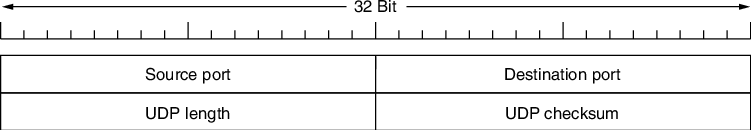
\includegraphics[width=0.6\textwidth]{images/header_udp.png}
\end{center}
I primi due campi indicano la porta del mittente e quella del destinatario e servono appunto per consegnare il segmento al corretto processo.\\
Nel campo \textit{UDP length} indica la lunghezza dell'intero segmento, ovvero header e payload espressa in byte. Il numero massimo è 65515 e non 65535 a causa del limite di dimensione imposto sui pacchetti IP.\\
Infine c'è un campo \textit{checksum} opzionale (raramente utilizzato) calcolato con somme in complemento a uno.\\\\
Il protocollo non si occupa quindi di controllo di flusso, del controllo di congestione e della ritrasmissione dopo la mancata consegna di un segmento. Questi compiti sono lasciati al livello applicazione.\\
Viene utilizzato nel DNS e nelle applicazioni di streaming video.

\subsection{TCP - Transmission Control Protocol}
Al contrario di tutti i protocolli Internet visti fin'ora, questo qui è orientato alla connessione e si occupa di fornire un flusso di byte affidabile end-to-end. Si occupa quindi di controllo dell'errore, gestione dei flussi al fine di evitare le congestioni e ritrasmissione in caso di mancata consegna. Esiste quindi un canale full-duplex virtuale da un punto A ad un punto B con TCP.

\subsubsection{Header TCP}
\begin{minipage}{0.4\textwidth}
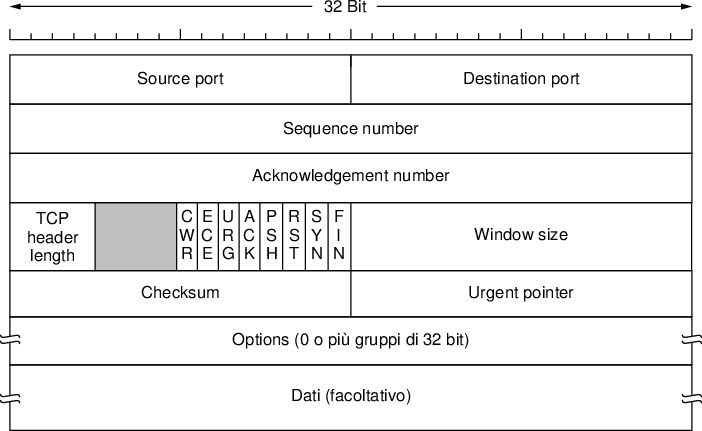
\includegraphics[width=\textwidth]{images/header_tcp.png}
\end{minipage}
\begin{minipage}{0.6\textwidth}
L'header inizia come in UDP con le due porte di mittente e destinatario. Successivamente ci sono \textit{sequence number e acknowledgment number} che servono per il controllo di flusso con sliding window ad ampiezza variabile.\\
Il campo \textit{header length} indica quanti gruppi di 32 bit sono contenuti nell'intestazione TCP, necessario visto che il campo \textit{options} opzionale ha lunghezza variabile a multipli di 32 bit.\\
Segue un campo di 4 bit inutilizzato, inseriti per eventuali correzioni o modifiche al protocollo. Seguono 8 bit di controllo spiegati in seguito. Successivamente troviamo il campo \textit{window size}, che indica l'ampiezza della sliding window. Infine il campo \textit{checksum} effettua il controllo dell'errore con semplici somme in complemento a uno.
\end{minipage}

\begin{itemize}
\item \textit{CWR ed ECE} sono utilizzati per segnalare la congestione
\item \textit{URG} segnala che il segmento contiene dati urgenti. Se a 1 nel campo \textit{urgent pointer} vi sarà lo spiazzamento in byte ai dati urgenti nel payload. Viene utilizzato raramente
\item \textit{ACK} indica che c'è ACK in piggyback
\item \textit{PSH} sta per PUSH e chiede gentilmente al destinatario di consegnare subito i dati al livello applicazione e di non archiviarli nel buffer
\item \textit{RST} significa reset e serve a resettare una connessione che risulta confusa per varie ragioni (malfunzionamento etc...). Utilizzato anche per rifiutare un segmento invalido o un tentativo di aprire una connessione
\item \textit{SYN} viene utilizzato per aprire la connessione tramite handshake a 3 vie
\end{itemize}

\subsubsection{Instaurazione di una connessione TCP}
\begin{minipage}{0.3\textwidth}
\begin{center}
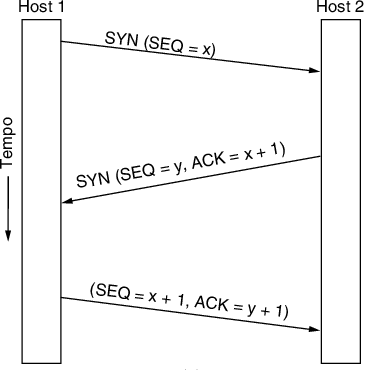
\includegraphics[width=\textwidth]{images/handshake.png}
\end{center}
\end{minipage}
\begin{minipage}{0.7\textwidth}
L'apertura di una connessione in TCP avviene tramite il \textbf{3-way-handshake}.\\
Questo metodo prevede un triplo scambio di pacchetti per avviare una connessione in modo da evitare duplicati.\\
Un lato (host 2) attende in modo passivo la connessione in ingresso, mentre l'altro (host 1) esegue una primitiva CONNECT specificando l'indirizzo IP e la porta a cui vuole connettersi, oltre che alla sua sequenza. Quest'ultima è un numero che aumenta lentamente e serve appunto per identificare una connessione ed evitare i duplicati.
La primitiva invia un segmento TCP con bit SYN a 1 e il bit ACK a 0, attendendo poi la risposta.\\
L'host 2 a questo punto controlla se ci sono processi che hanno eseguito la primitiva LISTEN su quella determinata porta, in caso negativo rispondono con un segmento con il bit RST a 1. Se accetta, invece, viene restituito un segmento di ACK, annunciando inoltre il suo numero di sequenza iniziale. Infine viene inviato un ACK da host 1 a host 2 confermando la sequenza ricevuta e la connessione è stabilita.
\end{minipage}

\subsubsection{Rilascio di una connessione TCP}
\begin{minipage}{0.7\textwidth}
Il rilascio della connessione deve avvenire in modo simmetrico per evitare la perdita di dati, al contrario del sistema telefonico in cui avviene in modo asimmetrico (basta che uno dei due riagganci per chiudere la connessione). Ci si comporta quindi come se esistessero due connessioni unidirezionali. Uno dei due host invia un segmento DISCONNECTION REQUEST - DR per avviare la procedura di rilascio. L'altro host, se non ha nemmeno lui più nulla da trasmettere, invia a sua volta un segmento DR ed avvia un timer. Il mittente originale, ricevuto questo DR, invia l'ACK e termina la connessione. All'arrivo dell'ACK anche il secondo host termina la connessione. Nel caso in cui questo segmento vada perso scatta il timeout e rilascia la connessione comunque.\\
Anche il primo host avvia un timer quando invia il DR, tuttavia se scatta il timeout non rilascia la connessione ma invia di nuovo la richiesta. Se dopo $N$ timeout non riceve risposta significa che qualcosa non va e rilascia la connessione.
\end{minipage}
\begin{minipage}{0.3\textwidth}
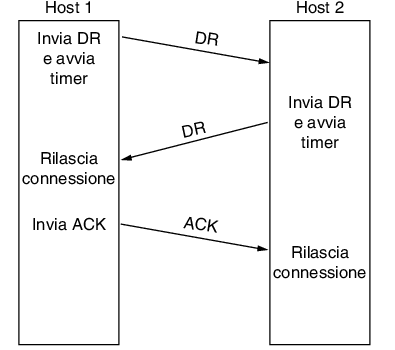
\includegraphics[width=\textwidth]{images/rilascio_connessione.png}
\end{minipage}
\newpage
\section{Livello applicazione}
A questo livello si trovano di fatto le applicazioni utente. Durante il corso ne è stata analizzata solamente una e molto brevemente, il DNS.

\subsection{DNS - Domain Name System}
Ogni macchina in rete è identificata tramite il suo indirizzo IP (che poi sia nattato con una porta a livello di rete è un altro discorso). Tuttavia è più facile memorizzare dei nomi piuttosto che dei numeri. DNS serve appunto per associare un indirizzo mnemonico, ad un indirizzo numerico. È un database distribuito in più parti di internet che effettua questa associazione secondo uno schema gerarchico.

\subsubsection{Lo spazio dei nomi DNS}
\begin{center}
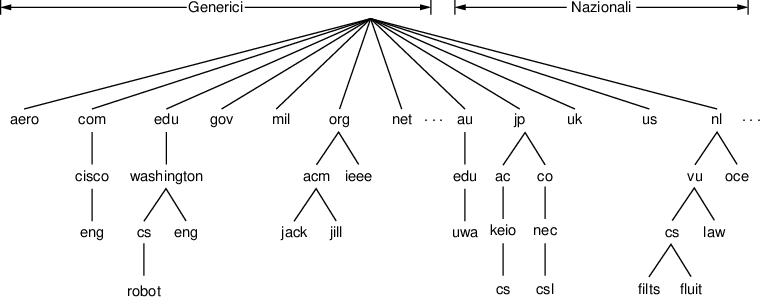
\includegraphics[width=0.7\textwidth]{images/dns.png}
\end{center}
In cima alla gerarchia di assegnazione dei nomi c'è l'associazione ICANN. Internet è divisa in oltre 250 domini di primo livello (.com, .it, .org, etc...), che possono essere generici o per nazioni.\\
I domini di secondo livello possono essere invece acquistati da chiunque e sono gestiti da \textit{registrar}, delegata da ICANN.\\
I nomi di dominio non sono case sensitive e ogni componente può essere lungo fino a 63 caratteri, mentre il percorso completo non può superare i 255 caratteri. Per creare un nuovo dominio è necessaria l'autorizzazione del dominio in cui sarà incluso.\\\\
A ogni dominio viene associato un record del database con i seguenti valori:
\begin{itemize}
\item \textit{domain name}: indica il nome del dominio a cui si riferisce il record
\item \textit{time to live}: offre un'indicatore della stabilità del record (information fading)
\item \textit{class}: per le informazioni che riguardano Internet è sempre \textit{IN}
\item \textit{type}: specifica il tipo di record
\item \textit{value}: contiene l'indirizzo IP vero e proprio della risorsa
\end{itemize}

\subsubsection{Name server}
Sono i dispositivi che di fatto contengono il database. Lo spazio dei nomi DNS viene diviso in zone non sovrapposte. Ognuna di essere contiene alcune parti della struttura ad albero. Per ogni zona vi è uno o più name server.\\
Il processo di ricerca di un nome e di un indirizzo è chiamato \textit{name resolution} ed avviene in modo ricorsivo: si interroga prima il name server della rete locale (solitamente il router); se questo ha l'informazione che cerchiamo ci invia la risposta, altrimenti interroga a sua volta il name server a livello più alto e così via. L'informazione viene inoltre mantenuta dai name server a livello più basso per ottimizzare le ricerche per un determinato lasso di tempo che viene rinnovato ogni volta che viene richiesta quella tupla (information fading).

\section{Sicurezza nelle reti}
Questo campo nasce al livello applicazione per rimediare alla totale assenza di sicurezza nei livelli inferiori, visto che sono nati per essere utilizzati in ambito militare in un ambiente closed-world.

\subsection{Crittografia}
Con \textit{crittografia} si intende il processo mediante il quale si rendono illeggibili determinate informazioni a chiunque non sia il destinatario designato. Quest'ultimo effettuerà la \textit{decifrazione} secondo un preciso algoritmo usando la chiave.\\
Nel caso in cui venga fatta una forzatura per rompere la crittografia si parla di \textit{decriptare}, viene eseguita da un \textit{criptoanalista}.\\\\
Essa nasce nel 1883 in ambito militare. \textbf{Kerckhoff} ne definì i principi fondamentali.
\begin{enumerate}
\item Il sistema dovrebbe essere inviolabile, in pratica anche se non in teoria.
\textbf{\item Il design di un sistema non dovrebbe richiedere segretezza, è la chiave ad esserlo.}
\item La chiave dovrebbe essere memorizzabile anche senza dover essere scritta.
\item I crittogrammi dovrebbero essere trasmissibili tramite telegrafo (obsoleto - non più valido).
\item L'apparato crittografico e i documenti dovrebbero essere portatili e gestiti da una sola persona (obsoleto).
\item Il sistema dovrebbe essere facile ed efficace.
\end{enumerate}
Esistono due tipi di crittografia:
\begin{itemize}
\item a \textbf{cifrario}, ovvero una trasformazione carattere per carattere senza considerare la struttura linguistica del messaggio
\item a \textbf{codice}, in cui si rimpiazza ogni parola con un'altra parola o simbolo. Questa tecnica non è più utilizzata
\end{itemize}

\subsubsection{Tipi di attacco}
In base alle informazioni che ha il criptoanalista si distinguono 3 tipi di attacco.
\begin{itemize}
\item \textbf{Cipher text only:} l'attaccante conosce solo il testo cifrato. È il metodo più difficile per rompere un algoritmo di crittografia.
\item \textbf{Known plaintext:} oltre a conoscere il testo cifrato, si conosce il relativo testo in chiaro. In questo modo si hanno più possibilità di successo.
\item \textbf{Chosen plaintext:} rappresenta il caso in cui l'attaccante ha tutte le informazioni possibili eccetto la chiave di decifratura. Può ottenere un testo cifrato per ogni relativo testo in chiaro.
\end{itemize}
L'importante è non sottovalutare mai l'attaccante e supporre che abbia il più alto grado di conoscenza.

\subsubsection{Cifrari a sostituzione}
Il primo cifrario di questo tipo è il \textit{cifrario di Cesare}, in cui ogni lettera viene spostata in avanti secondo la sequenza dell'alfabeto. Una generalizzazione è spostare le lettere di $k$ volte nell'alfabeto.\\
Un metodo ancora più efficace è quello di associare ogni lettera ad un'altra secondo un preciso schema segreto.\\
Queste tecniche prendono il nome di \textbf{sostituzione monoalfabetica}.\\
Tuttavia non è più sicura in quanto è possibile romperla conoscendo il linguaggio in cui è scritto il messaggio originale.\\
Ogni linguaggio ha delle lettere, digrammi e trigrammi che si ripetono più frequentemente di altri (ad esempio in inglese la lettera e si ripete più frequentemente di tutte, th tra i digrammi e the tra i trigrammi). Procedendo per tentativi, analizzando il carattere o gruppi di caratteri che si ripetono più volte è possibile ricostruire lo schema associativo utilizzato per la cifratura.
Questo attacco si chiama \textit{analisi di frequenza}.\\
Un altro approccio consiste nell'indovinare una parola o una frase che probabilmente si trovano dentro il testo se, oltre al linguaggio, si conosce il contesto della comunicazione. 

\subsubsection{Cifrari a trasposizione}
Questo tipo di cifrari, al contrario dei precedenti, riordinano le lettere senza mascherarle. Un esempio è il \textit{cifrario a trasposizione colonnare} mostrato in figura.
\begin{center}
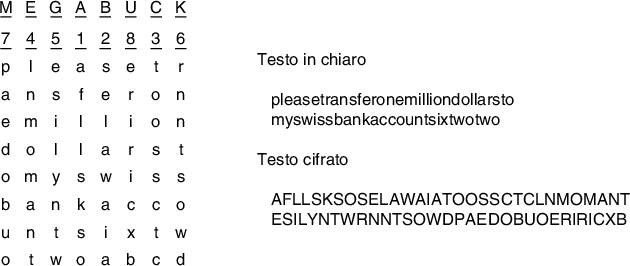
\includegraphics[width=0.6\textwidth]{images/cifrario_trasposizione.png}
\end{center}
Il testo in chiaro viene scritto orizzontalmente, per righe, fino a riempire la matrice, eventualmente aggiungendo caratteri non significativi. Il testo cifrato viene letto per colonna, cominciando con quella che ha la lettera chiave più bassa.\\
Ora basare l'attacco sulle statistiche dei linguaggi naturali non è efficace.\\
La macchina Enigma usava anche questa tecnica mescolata con la precedente.\\
Per rompere la cifratura in questo caso è necessario prima di tutto riconoscere che il testo è stato trasposto e non mascherato. È facile accorgersene in quanto ogni lettera rappresenta se stessa e la distribuzione di frequenza rimane intatta. Nel caso in cui le lettere siano anche sostituite è necessario ricondursi al metodo per rompere i cifrari a sostituzione e successivamente applicare queste tecniche.\\
Poi si fa un'ipotesi sul numero di colonne: in molti casi si riesce ad indovinare dal contesto di una parola o frase che con buona probabilità appaiono nel testo.\\
Il passo conclusivo consiste nel trovare l'ordine delle colonne. Se vi sono $k$ colonne ci saranno $k!$ possibilità, tuttavia si possono riordinare come quando si fa un puzzle, ricomponendo pezzi di parole o di frasi.

\subsubsection{OTP One-Time-Pad}
Il cifrario a \textit{blocchi monouso} è l'unico sicuro al 100\%, tuttavia è irrealizzabile.\\
In pratica consiste nel combinare in XOR i bit del messaggio originale con una sequenza pseudocasuale di bit lunga quanto il messaggio (OTP). Effettuando nuovamente la XOR tra il messaggio cifrato e la stessa sequenza pseudocasuale si effettua la decifratura. Una volta utilizzata, l'OTP va distrutta e mai più usata per cifrare messaggi, altrimenti si perderebbe il 100\% di sicurezza.
\begin{center}
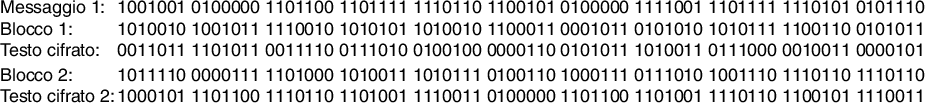
\includegraphics[width=0.7\textwidth]{images/otp.png}
\end{center}
In questo modo, senza la chiave, l'unica alternativa che rimane all'attaccante è il brute force, impraticabile con le velocità degli elaboratori moderni.\\
Tuttavia questo metodo richiede che l'OTP sia memorizzato fisicamente da qualche parte, e deve essere mandato al destinatario, generando una falla di sicurezza.\\
Anche nel caso in cui mittente e destinatario possiedano le stesse OTP ci potrebbe essere un problema di perdita di sincronizzazione o caratteri persi o inseriti per sbaglio. In questi casi il messaggio sarebbe indecifrabile anche conoscendo le OTP.

\subsection{Algoritmi simmetrici a chiave condivisa}
Chiave simmetrica significa che la stessa chiave viene usata dagli algoritmi di cifratura e decifratura.\\
In particolare, un tipo di questi algoritmi, sono i \textit{cifrari a blocco}, che prendono $n$ bit dal testo in chiaro e li trasformano usando la chiave in $n$ bit cifrati. Possono essere realizzati in hardware, per aumentare la flessibilità, o via software, per aumentarne la flessibilità. Sono realizzati mediante la combinazione ripetuta di due componenti fondamentali:\\\\
\begin{minipage}{0.7\textwidth}
\begin{itemize}
\item \textbf{P-BOX:} la \textit{permutation box} effettua semplicemente permutazioni dei bit in ingresso facendoli passare tramite le sue linee interne. La trasposizione è praticamente istantanea se avviene a livello hardware, visto che non c'è nessun calcolo da eseguire.
\item \textbf{S-BOX:} la \textit{serial box} sostituisce una sequenza di bit in input con una diversa in output della stessa lunghezza secondo un preciso schema. I 3 bit in input scelgono una delle 8 linee che escono dal primo stadio e le impostano a 1, tutte le altre sono a 0. Il secondo stadio è una P-BOX. Il terzo stadio codifica le linee di input selezionate riportandole in binario.
\end{itemize}
\end{minipage}
\begin{minipage}{0.3\textwidth}
\begin{flushright}
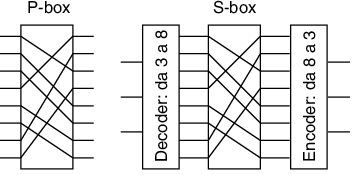
\includegraphics[width=0.9\textwidth]{images/p-s-box.png}
\end{flushright}
\end{minipage}

\subsubsection{DES e triplo DES}
Il \textit{Data Encryption Standard} è stato il primo standard di sicurezza applicato alle reti di computer. È stato commissionato alla IBM dal governo degli Stati Uniti. Inizialmente aveva il nome di Lucifer, prevedeva chiavi a 128 bit. Tuttavia l'intelligence statunitense voleva renderlo vulnerabile in modo che solo loro potessero violarlo nel caso avessero avuto bisogno, dunque ridussero la chiave a 56 bit. Con l'aumentare della potenza di calcolo dopo alcuni anni DES venne violato.\\
L'algoritmo lavora su blocchi da 64 bit ed effettua 19 passaggi per criptare. Una peculiarità di DES è che effettuare in successione cifratura e decifratura o viceversa da in output il testo in chiaro. Definendo come $E$ il processo di encrypting e $D$ quello di decrypting è vero che $P=E(D(P))=D(E(P))$ dove $P$ è il testo in chiaro.\\\\
3DES nasce per tappare la falla di sicurezza creata dalla riduzione della chiave a 56 bit; deve essere inoltre retrocompatibile con tutti i dispositivi già prodotti e venduti per supportare DES.
\begin{center}
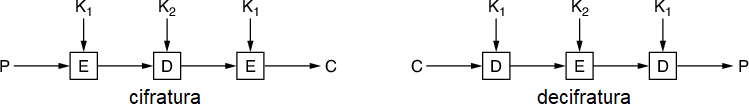
\includegraphics[width=0.7\textwidth]{images/3DES.png}
\end{center}
La strategia non è quella di effettuare 3 volte l'encrypting, poiché perderebbe la caratteristica fondamentale di retrocompatibilità. Si usano 2 chiavi da 56 bit, $k_1$ e $k_2$, dunque la potenza è elevata al quadrato rispetto a DES visto che la chiave è doppia (112 bit). I procedimenti eseguiti sono quelli in figura. Se scegliamo $k_1=k_2$ allora l'algoritmo diventa automaticamente DES.

\subsubsection{AES}
3DES durò per circa 20 anni, poi venne bandito un concorso mondiale che chiedeva un algoritmo di crittografia nuovo. I vincitori furono due ricercatori belgi, crearono Rijndael che prese il nome commerciale di \textit{AES - Advanced Encryption Standard}. Utilizza blocchi e chiavi da 128 o 256 bit, P-BOX ed S-BOX.

\subsubsection{Blowfish e Twofish}
Un altro cifrario a blocchi nato prima di AES è blowfish ed è tutt'ora inviolato. Lavora su blocchi a 64 bit con chiavi da 32 a 448 bit. Tuttavia era più lento di AES perciò non ebbe successo. Il suo successore, twofish, superava questo problema lavorando su blocchi da 128 bit con chiavi da 128 a 256 bit, tuttavia AES aveva già preso piede.

\subsection{Modalità di cifratura}
Tutti gli algoritmi sopra soffrono di un grave problema di sicurezza: la stessa chiave viene usata per cifrare tutti i blocchi. Un intruso può usare questa proprietà per forzare il cifrario.

\subsubsection{ECB - Electronic Code Book}
La modalità d'impiego più ovvia del DES (o altri) per cifrare un lungo testo in chiaro consiste nel suddividerlo in blocchi di 64 bit, che vengono cifrati uno dopo l'altro con la stessa chiave. L'ultimo pezzo può essere finito con del padding se troppo corto. Questa tecnica prende il nome di ECB ed è la più insicura, in quanto l'attaccante può spostare blocchi di testo cifrato senza conoscerne il contenuto, noi non potremmo accorgercene se il file fosse un eseguibile ad esempio.

\subsubsection{*Cipher Block Chaining}
Per evitare gli attacchi sopra descritti si collegano tutti i blocchi cifrati in diversi modi, così quando si tenta di spostare interi blocchi la fase di decoding fallisce e ci accorgiamo della corruzione dei dati.\\
Per ottenere questo effetto ogni blocco di testo in chiaro è messo in XOR con il precedente blocco cifrato prima di eseguire la cifratura vera e propria. Il primo blocco è messo in XOR con un vettore di inizializzazione, il quale verrà trasmesso in chiaro per effettuare il decoding con le operazioni inverse (XOR e decoding).
\begin{center}
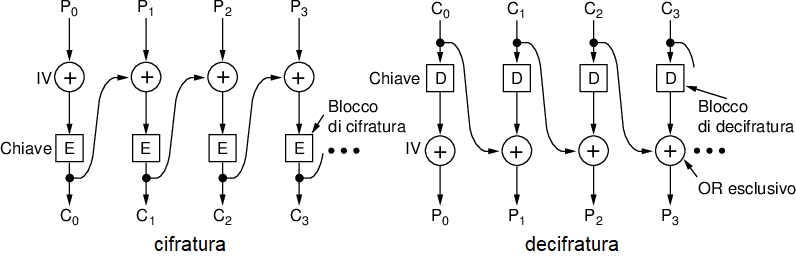
\includegraphics[width=0.7\textwidth]{images/cipher_block_chaining.png}
\end{center}

\subsubsection{Stream Cipher}
\begin{minipage}{0.4\textwidth}
Il cifrario a flusso utilizza un vettore di inizializzazione come nel caso precedente con una chiave crittografica per ottenere il primo blocco in uscita. Quest'ultimo viene cifrato per ottenere il secondo, che a sua volta viene cifrato per avere il terzo e così via. Viene trasmesso il risultato e il vettore di inizializzazione per eseguire la decifratura seguendo i passaggi inversi.
\end{minipage}
\begin{minipage}{0.5\textwidth}
\begin{flushright}
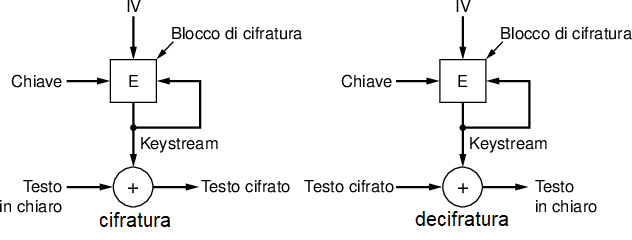
\includegraphics[width=\textwidth]{images/stream_cipher.png}
\end{flushright}
\end{minipage}

\subsubsection{*Counter}
\begin{minipage}{0.7\textwidth}
Un problema comune a tutte le precedenti modalità di cifratura è che per accedere ai dati in modo casuale è necessario decifrarli tutti (molto scomodo). Perciò è stata inventata questa modalità: il testo in chiaro viene messo in XOR con un vettore di inizializzazione che viene cifrato. Il testo del blocco successivo viene messo in XOR con il vettore di inizializzazione incrementato di uno e così via. Avendo quindi il vettore originale e la chiave è facile decifrare il blocco desiderato aggiungendo uno spiazzamento al vettore.
\end{minipage}
\begin{minipage}{0.3\textwidth}
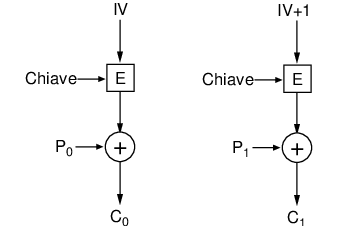
\includegraphics[width=\textwidth]{images/counter.png}
\end{minipage}

\subsubsection{Keystream reuse attack}
Supponendo di cifrare due messaggi con lo stesso vettore di inizializzazione con uno dei metodi precedenti sorge una vulnerabilità.\\
Avremo quindi due messaggi cosi cifrati:\\
$P1 \oplus k=C1$\\
$P2 \oplus k=C2$\\
$C1 \oplus C2=P1 \oplus k \oplus k \oplus P2=P1 \oplus P2$, ovvero lo xor tra i due messaggi in chiaro. Ecco che quindi si possono attuare tutte le tecniche viste in precedenza di analisi di frequenza basata sul linguaggio o usare il contesto della comunicazione se lo si conosce.

\subsubsection{Reply attack}
Un altro attacco attuabile se un mittente utilizza due volte lo stesso vettore di inizializzazione è \textit{l'attacco a ripetizione}: l'attaccante manda un messaggio con lo stesso vettore di inizializzazione, causando effetti collaterali poiché si finge il mittente originale anche senza conoscere il contenuto, semplicemente replica pacchetti già immessi nella rete. Usato in vecchi videogiochi online per lanciare più volte lo stesso oggetto o utilizzare più volte lo stesso elemento in generale.

\subsection{Algoritmi asimmetrici a chiave pubblica - RSA}
Il problema maggiore degli algoritmi simmetrici è come far arrivare la chiave al destinatario senza che venga intercettata da terzi. Per farlo si cifra la chiave con questi algoritmi asimmetrici, i quali non richiedono la segretezza della chiave.\\
Un esempio è RSA, che si basa su alcuni principi della teoria dei numeri. Se l'host Alice deve comunicare con l'host Bob sceglie due numeri grandi primi $p$ e $q$, calcolandone il prodotto. Quest'ultimo viene mandato a Bob che usa $p\cdot q$ per codificare la chiave dell'algoritmo simmetrico. Per eseguire la decodifica è necessario avere $p$ e $q$ separati, l'unica ad averli è Alice. Ora possiedono entrambi la stessa chiave e possono usare uno dei qualsiasi algoritmi visti prima.\\
In \textit{RSA-X} il livello di sicurezza cresce esponenzialmente all'aumentare di $x$, che indica il numero di cifre che compongono il prodotto $p\cdot q$. L'algoritmo è tutt'ora inviolabile in quanto è impossibile matematicamente fattorizzare un numero che abbia come unici due fattori due numeri così grandi.

\subsection{Firma digitale asimmetrica con chiave pubblica}
Il problema maggiore in rete, dopo la segretezza, è l'autenticazione del mittente. Per farlo con gli algoritmi asimmetrici, i quali hanno funzioni di criptazione (E) e decriptazione (D) inverse, si procede in questo modo: Alice prende il messaggio in chiaro P e lo decripta con la sua chiave privata; lo cripta successivamente con la chiave pubblica di Bob.\\
Quest'ultimo decripta il messaggio con la sua chiave privata e verifica il mittente criptandolo con la chiave pubblica di Alice.\\
Tuttavia questa operazione richiede molto overhead, perciò se non abbiamo bisogno della sicurezza è inutile firmare tutto il messaggio.\\
Viene quindi calcolato il \textbf{message digest} o \textbf{hash crittografico}, il quale è una compressione del messaggio originale. Quest'ultimo viene firmato con la chiave privata del mittente. Il ricevente verifica la firma con la chiave pubblica, ricalcola l'hash del messaggio con lo stesso algoritmo (SHA, MD5, etc...) e li confronta.\\
Le caratteristiche che possiedono gli hash e che garantiscono l'affidabilità di questo metodo sono le seguenti:
\begin{enumerate}
\item Dato un plaintext P è relativamente semplice calcolare il suo hash
\item Dato un $P$ è difficilissimo trovare $P' \neq P$ tale che hash(P)=hash(P')
\item Dato hash(P) è praticamente impossibile trovare P
\item Piccole modifiche sul testo P provocano enormi cambiamenti su hash(P)
\end{enumerate}

\subsection{Firma digitale simmetrica con chiave condivisa}
In questo metodo si calcola l'\textbf{HMAC} del messaggio (Hashed Message Authentication Code), che corrisponde all'hash del messaggio seguito dalla chiave, hash(messaggio, chiave)=H.\\
H viene inviato insieme al messaggio in chiaro. Solamente avendo la stessa chiave si può ricreare lo stesso hash a partire dal messaggio in chiaro.\\
Viene usato in \textbf{IPsec}, ovvero la versione sicura di IP. Ecco la sua intestazione.
\begin{center}
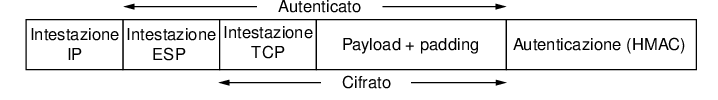
\includegraphics[width=0.7\textwidth]{images/ipsec.png}
\end{center}
ESP (Encapsulating Security Payload) fornisce un controllo di integrità HMAC.\\
IPsec viene usato nelle \textbf{VPN} (Virtual Private Network), dove prima si crea una chiave segreta condivisa, usata per generare gli HMAC. Tutti i messaggi vengono verificati ricalcolando l'hash.

\subsection{Attacchi alla sicurezza di un sistema informatico}
\subsubsection{Attacco MITM - Man In The Middle}
\begin{minipage}{0.45\textwidth}
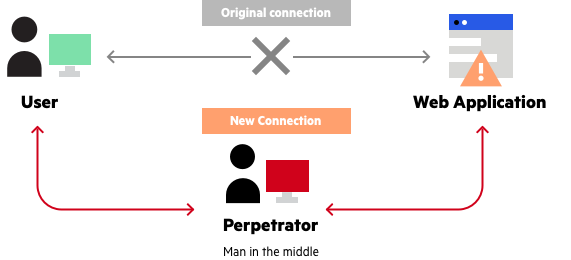
\includegraphics[width=\textwidth]{images/mitm.png}
\end{minipage}
\begin{minipage}{0.55\textwidth}
Questa tecnica prevede l'interruzione del collegamento originale; i pacchetti vengono dirottati in un nuovo canale che attraversa l'attaccante. Rende impossibile la gestione della sicurezza simmetrica senza informazione pre-condivisa. Un possibile metodo per realizzarla è l'\textbf{ARP spoofing} o \textbf{ARP poisoning}, ovvero sfruttare la falla di sicurezza del protocollo ARP che permette di rispondere a richieste non a noi indirizzate: quando una macchina chiede chi abbia un certo indirizzo IP all'interno della LAN possiamo rispondere con il nostro MAC anche se il nostro IP non è quello. In questo modo tutto il traffico diretto a quel indirizzo IP (ad esempio il sito della banca) viene dirottato a noi, che provvederemo a salvarlo e ad inoltrarlo al sito originale, ripetendo poi la conseguente risposta.
\end{minipage}\\\\
Per superare questo tipo di attacchi è necessario fare un atto di fede verso le \textbf{CA} (Certification Authority), le quali rilasciano certificati per i siti web in modo che siano autenticati. Si possono usare poi gli algoritmi di firma digitale asimmetrica, dove la chiave pubblica viene inviata dentro al certificato della CA.\\
Dentro ai sistemi operativi ci sono già dei certificati embedded, in modo da garantire le prime connessioni. Installare sistemi operativi provenienti da fonti non certe espone l'utente ad un altissimo rischio.

\subsubsection{Denial of Service - DoS}
Questo tipo di attacchi puntano a far esaurire le risorse di chi fornisce un certo servizio in modo da renderlo non disponibile.
\begin{itemize}
\item \textbf{SMURF:} vengono mandati pacchetti ICMP chiedendo l'ECHO, detto anche \textit{ping of death}.
\item \textbf{SYN Attack:} vengono inviati molti pacchetti per aprire una connessione TCP con un certo server. Quest'ultimo risponde con l'ACK come previsto dal protocollo 3-way handshake implementato in TCP, attendendo la terza stretta di mano che mai arriverà. Arriveranno invece molte altre richieste di apertura connessione finché la memoria non è satura, il server inizierà quindi a rifiutare nuove connessioni, comprese quelle degli utenti reali.
\item \textbf{DDoS:} Distributed DoS è DoS all'ennesima potenza. Teoricamente abbiamo bisogno di molte macchine zombie (sotto il nostro controllo) che attaccano contemporaneamente il server remoto. Nella pratica, vista la mancanza di sicurezza in IP, vengono inviati pacchetti ICMP a molte macchine inserendo nel campo indirizzo mittente l'IP del server da attaccare. In questo modo tutte le macchine che ricevono questo ICMP rispondono con l'ECHO al server.
\end{itemize}

\subsubsection{DNS attack}
I server DNS fanno parte dell'infrastruttura critica di internet, visto che se si riuscisse a modificare le tuple del database distribuito si potrebbe generare caos (ad esempio se l'indirizzo google.com venisse associato ad un IP che non appartiene a Google ogni volta che si digita quell'indirizzo mnemonico si verrebbe mandati su un sito che non ha niente a che vedere). Esistono diversi tipi di attacco ai DNS:
\begin{itemize}
\item \textbf{DNS amplification:} si fa un DDoS contro i name server mandandoli down e oscurando difatto siti che non lo sono in una certa area del mondo (più alto è il livello del DNS abbattuto e più vasta sarà l'area colpita)
\item L'alternativa è alterare i dati del server DNS in modo da indirizzare gli utenti dove vogliamo. È necessario fare tapping sul DNS vero, altrimenti arriveranno due risposte e il richiedente si accorgerà della discrepanza.
\end{itemize}
Inizialmente vennero introdotti numeri di sequenza nelle richieste DNS allegati in chiaro, tuttavia è un metodo troppo insicuro in quanto è sufficiente clonare questo numero: ad esempio un utente chiede un IP ad un DNS, il quale inoltra la richiesta ad un name server di livello superiore. L'utente prontamente risponde clonando il numero di richiesta con un IP fasullo.\\
Viene quindi introdotta la firma digitale in DNS. Ne deriva il problema dell'autenticazione iniziale, risolta precedentemente con le certification authority. Vengono introdotti quindi i \textbf{root server}, super sicuri di cui gli altri name server si fidano ciecamente. Sono 13 in tutto il mondo e vengono replicati fino ad arrivare a poco più di 1000 macchine root.\\
Le chiavi di questi server sono di lunghezza media e vengono cambiate periodicamente. Se fossero troppo lunghe il sistema diventerebbe troppo lento. Le chiavi dei root server sono firmate con la  \textbf{KSK} (Key Signing Key). Quest'ultima è stata suddivisa in 7 parti, ognuna assegnata ad una persona diversa. Bastano 5 pezzi per ricomporre la chiave originale. Nel 2018 la KSK è stata cambiata a 2048 bit.
\end{document}
